% Manuale Admin Cadenza — generato da scripts/build-manuale-latex.js
% Compilare con: xelatex MANUALE_ADMIN.tex (consigliato per Unicode)
%                oppure pdflatex (gli emoji vengono mappati in testo neutro)
\documentclass[11pt,a4paper]{article}

\usepackage[utf8]{inputenc}
\usepackage[T1]{fontenc}
\usepackage{lmodern}
\usepackage[italian]{babel}
\usepackage[a4paper,top=22mm,bottom=22mm,left=18mm,right=18mm]{geometry}
\usepackage{graphicx}
\usepackage{xcolor}
\usepackage{tabularx}
\usepackage{longtable}
\usepackage{array}
\usepackage{colortbl}
\usepackage{enumitem}
\usepackage{float}
\usepackage{titlesec}
\usepackage{fancyhdr}
\usepackage{lastpage}
\usepackage{eurosym}
\usepackage{amssymb}
\usepackage{textcomp}
\usepackage[bookmarks=true,colorlinks=true,linkcolor={blue!60!black},urlcolor={blue!60!black},citecolor={blue!60!black}]{hyperref}
\usepackage{listings}

% --- Listings (code blocks) ---
\lstset{
  basicstyle=\ttfamily\small,
  breaklines=true,
  frame=single,
  framesep=4pt,
  rulecolor=\color{black!20},
  backgroundcolor=\color{black!3},
  columns=fullflexible,
  keepspaces=true,
  showstringspaces=false,
}

% --- Colori tabelle ---
\definecolor{tableheader}{HTML}{F1EEE5}

% --- Header/footer ---
\pagestyle{fancy}
\fancyhf{}
\fancyhead[L]{\small Cadenza · Manuale Amministratore v1.6}
\fancyhead[R]{\small 13 maggio 2026}
\fancyfoot[C]{\small\thepage{} / \pageref{LastPage}}
\renewcommand{\headrulewidth}{0.4pt}

% --- Titoli sezione con stile leggero ---
\titleformat{\section}
  {\Large\bfseries\color{black!85}}{\thesection}{0.7em}{}
\titlespacing*{\section}{0pt}{14pt}{8pt}
\titleformat{\subsection}
  {\large\bfseries\color{black!75}}{\thesubsection}{0.7em}{}
\titleformat{\subsubsection}
  {\normalsize\bfseries\color{black!60}}{\thesubsubsection}{0.7em}{}

% --- Imposta i path immagini (gli alt riferiscono screenshots/* dal docs/) ---
\graphicspath{{./}{screenshots/}}

% --- Quote/Blockquote più tenue ---
\renewenvironment{quote}
  {\begin{list}{}{%
      \setlength{\leftmargin}{8pt}%
      \setlength{\rightmargin}{8pt}%
      \setlength{\topsep}{6pt}%
      \setlength{\parsep}{0pt}}%
      \item\relax\color{black!75}\itshape}
  {\end{list}}

\setlength{\parindent}{0pt}
\setlength{\parskip}{6pt}

% --- Frontmatter ---
\title{Cadenza --- Manuale Amministratore}
\author{Danilo Russo, docente del Conservatorio}
\date{13 maggio 2026}

\begin{document}

\maketitle
\thispagestyle{fancy}

\tableofcontents
\clearpage

\section*{Cadenza · Manuale Docente}
\addcontentsline{toc}{section}{Cadenza · Manuale Docente}


\begin{quote}
\textbf{Versione}: 1.0 · \textbf{Data}: 13 maggio 2026 · \textbf{Lingua}: italiano · \textbf{Formato stampa}: A4 \textbf{Destinatari}: docenti titolari, supplenti, contrattisti, collaboratori e accompagnatori del Conservatorio \textbf{Prerequisiti}: account su una installazione Cadenza già attiva (te lo crea la Segreteria o ti registri al primo accesso)
\end{quote}

\medskip\hrule\medskip

\section{Indice}


\begin{itemize}
  \item \href{\#1-in-due-minuti}{§1. In due minuti}
  \item \href{\#2-primo-accesso}{§2. Primo accesso}
  \item \href{\#3-dashboard-e-calendario}{§3. Dashboard e calendario}
  \item \href{\#4-prenotare-unaula}{§4. Prenotare un'aula}
  \item \href{\#5-le-tue-prenotazioni}{§5. Le tue prenotazioni}
  \item \href{\#6-check-in-con-qr-code}{§6. Check-in con QR code}
  \item \href{\#7-aule-e-dotazioni}{§7. Aule e dotazioni}
  \item \href{\#8-monte-ore--il-piano-annuale}{§8. Monte Ore — il piano annuale}
  \item \href{\#9-spostamenti-e-variazioni-dopo-lapprovazione}{§9. Spostamenti e variazioni dopo l'approvazione}
  \item \href{\#10-prestiti-strumenti}{§10. Prestiti strumenti}
  \item \href{\#11-avvisi-e-bacheca}{§11. Avvisi e bacheca}
  \item \href{\#12-profilo-notifiche-e-calendario-personale}{§12. Profilo, notifiche e calendario personale}
  \item \href{\#13-app-sul-telefono-pwa}{§13. App sul telefono (PWA)}
  \item \href{\#14-bot-telegram-opzionale}{§14. Bot Telegram (opzionale)}
  \item \href{\#15-lingue-dellinterfaccia}{§15. Lingue dell'interfaccia}
  \item \href{\#16-domande-ricorrenti}{§16. Domande ricorrenti}
\end{itemize}

\medskip\hrule\medskip

\section{1. In due minuti}


Cadenza è la piattaforma del Conservatorio per \textbf{prenotare le aule} e gestire il \textbf{Monte Ore annuale}. Da un'unica interfaccia puoi:

\begin{itemize}
  \item Prenotare studio, sala prove, sala concerti, aula didattica o ufficio.
  \item Compilare e inviare la tua \textbf{proposta Monte Ore} all'inizio dell'anno accademico.
  \item Chiedere \textbf{spostamenti} (cambio orario, cambio aula, sposta a un altro giorno) sulle lezioni già approvate.
  \item Richiedere \textbf{prestiti strumenti} dall'inventario dell'istituto.
  \item Leggere gli \textbf{avvisi} della Direzione filtrati per il tuo corso/ruolo.
  \item Ricevere \textbf{promemoria via email} prima di ogni lezione.
  \item Installare l'app \textbf{sul telefono} (Android e iPhone).
\end{itemize}

Cadenza è in italiano, inglese, spagnolo, tedesco e francese; cambia lingua dal tuo profilo.

\medskip\hrule\medskip

\section{2. Primo accesso}


\subsection{2.1 Login}


URL: \texttt{https://cadenza.tuoconservatorio.it/login} (l'URL esatto dipende dall'istituto --- chiedilo alla Segreteria).

\begin{figure}[H]\centering
\includegraphics[width=0.95\linewidth]{screenshots/login.png}\caption*{Schermata di login — scelta del provider o email + password}\end{figure}

Hai tre modi per entrare:

\begin{table}[H]
\centering
\small
\begin{tabularx}{\linewidth}{|X|X|}
\hline
\rowcolor{tableheader} Metodo & Quando usarlo \\
\hline
\textbf{Email + password} & Account creato dalla Segreteria; password ricevuta via email al primo invito. \\
\hline
\textbf{Google} & Se il Conservatorio ha attivato il login Google Workspace. \\
\hline
\textbf{Microsoft 365 / Entra ID} & Se il Conservatorio ha attivato il login Microsoft (account istituzionale). \\
\hline
\end{tabularx}
\end{table}


Click su "Email" apre il form classico:

\begin{figure}[H]\centering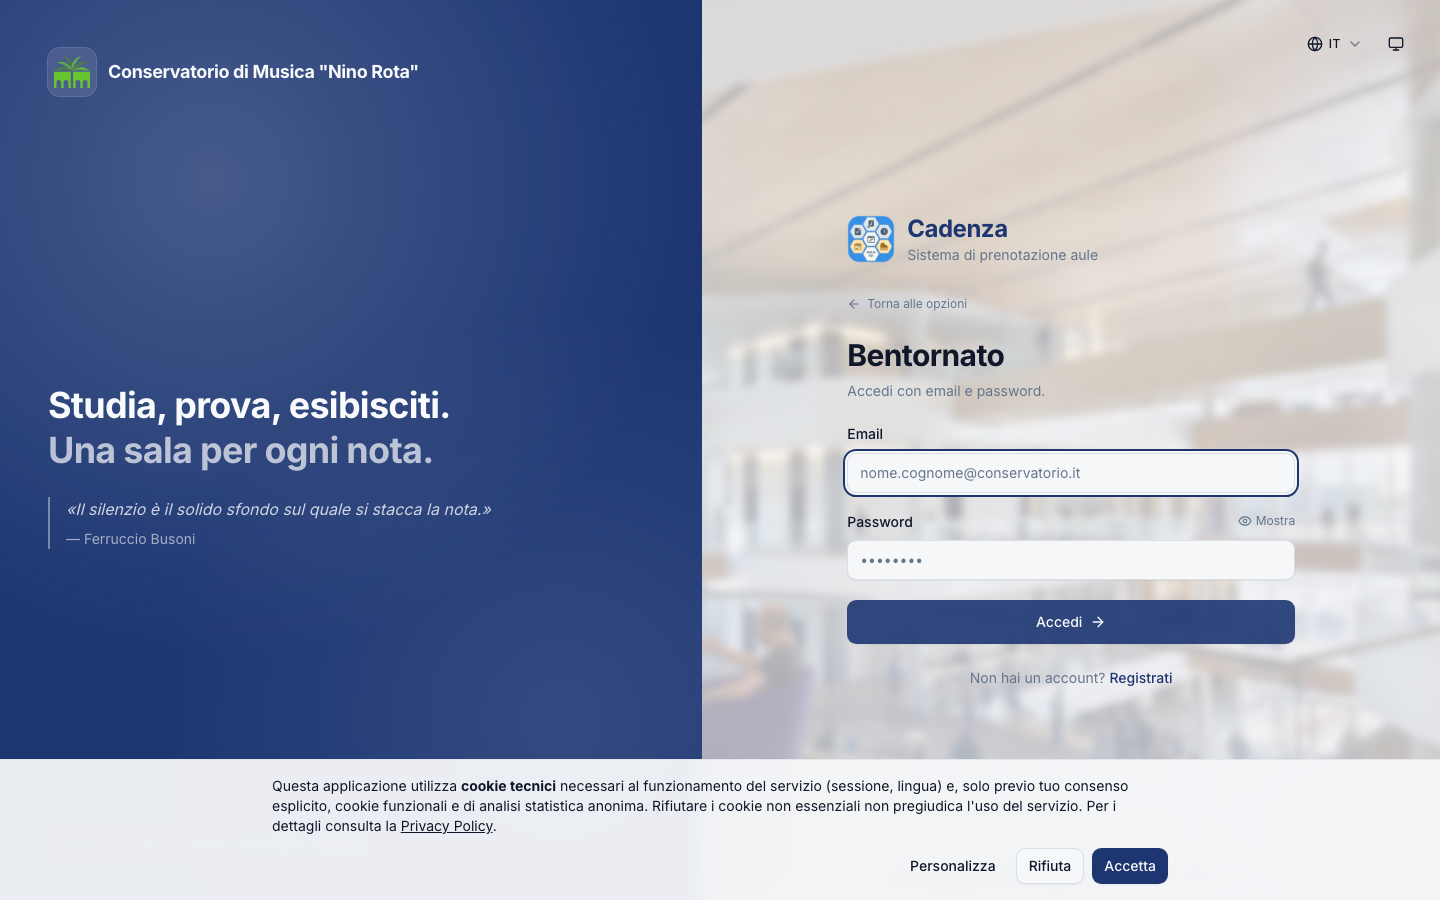
\includegraphics[width=0.95\linewidth]{screenshots/login-email.png}\caption*{Form email + password}\end{figure}

\begin{quote}
\textbf{2FA via email} (opt-in): se la Direzione lo attiva, dopo username/password riceverai un codice a 6 cifre. Inseriscilo per completare l'accesso. La 2FA è facoltativa per i docenti, \textbf{obbligatoria} per gli admin.
\end{quote}

\subsection{2.2 Cosa fare se non hai una password}


Se non hai mai ricevuto la password:

\begin{enumerate}
  \item Chiedi alla Segreteria di invitarti (ti arriverà via email un link).
  \item In alternativa, in fondo alla pagina di login c'è "Registrati": compila i tuoi dati e attendi che la Segreteria approvi il tuo account.
\end{enumerate}

\subsection{2.2-bis Password dimenticata}


Se hai la password ma non te la ricordi più, non serve la Segreteria --- risolvi da solo in 1 minuto:

\begin{enumerate}
  \item Apri la pagina di login.
  \item Sotto il bottone "Accedi", clicca su \textbf{"Password dimenticata?"}.
  \item Inserisci la tua email e clicca \textbf{"Invia link di reset"}.
  \item Riceverai entro pochi secondi un'email con un bottone "\textbf{Reimposta password}". Cliccalo (link valido \textbf{1 ora}, utilizzabile \textbf{una sola volta}).
  \item Scegli la nuova password (minimo 10 caratteri, almeno una maiuscola e un numero) e confermala.
  \item Vieni reindirizzato al login: accedi con la nuova password.
\end{enumerate}

\begin{quote}
\textbf{Sicurezza:} dopo il cambio password, \textbf{tutte le sessioni attive vengono disconnesse} (anche su altri dispositivi). Dovrai rifare il login ovunque. Se l'email non arriva entro qualche minuto, controlla lo spam o riprova dopo un po' (per evitare flood l'invio è limitato).  \textbf{Privacy:} se l'email che inserisci non corrisponde ad alcun account, il sistema ti mostra comunque "abbiamo inviato il link" --- è una scelta voluta per impedire a malintenzionati di scoprire quali email sono registrate.
\end{quote}

\subsection{2.3 Completamento del profilo (solo al primo accesso)}


Al primo login Cadenza ti chiede di completare l'anagrafica: nome, cognome, eventuale matricola, corso (se applicabile). Per i docenti il campo "corso" è facoltativo.

\begin{figure}[H]\centering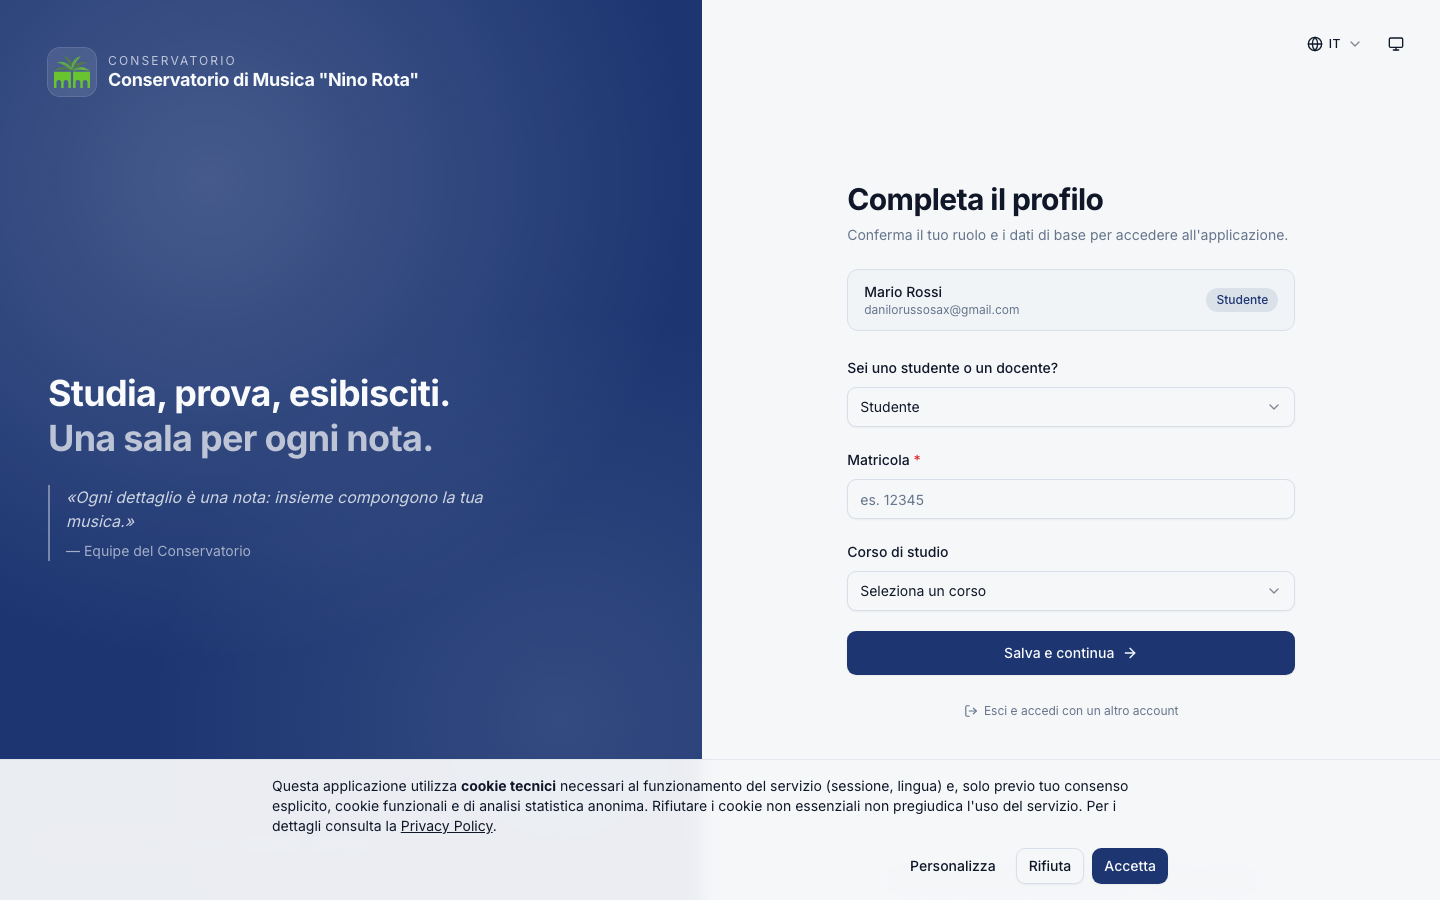
\includegraphics[width=0.95\linewidth]{screenshots/complete-profile.png}\caption*{Pagina di completamento profilo}\end{figure}

Dopo il completamento sei dentro e arrivi alla \textbf{Dashboard}.

\medskip\hrule\medskip

\section{3. Dashboard e calendario}


La Dashboard è la tua "home" dentro Cadenza. Mostra:

\begin{itemize}
  \item Il calendario delle aule del \textbf{giorno selezionato} (oppure di 3 giorni affiancati, vedi sotto).
  \item I tuoi \textbf{prossimi impegni} (Monte Ore + prenotazioni manuali) come elenco compatto.
  \item I \textbf{template di prenotazione rapida} ("Quick book") se ne hai salvato qualcuno.
  \item Gli avvisi importanti pubblicati dalla Direzione.
\end{itemize}

\subsection{3.1 Vista 1 giorno (default)}


\begin{figure}[H]\centering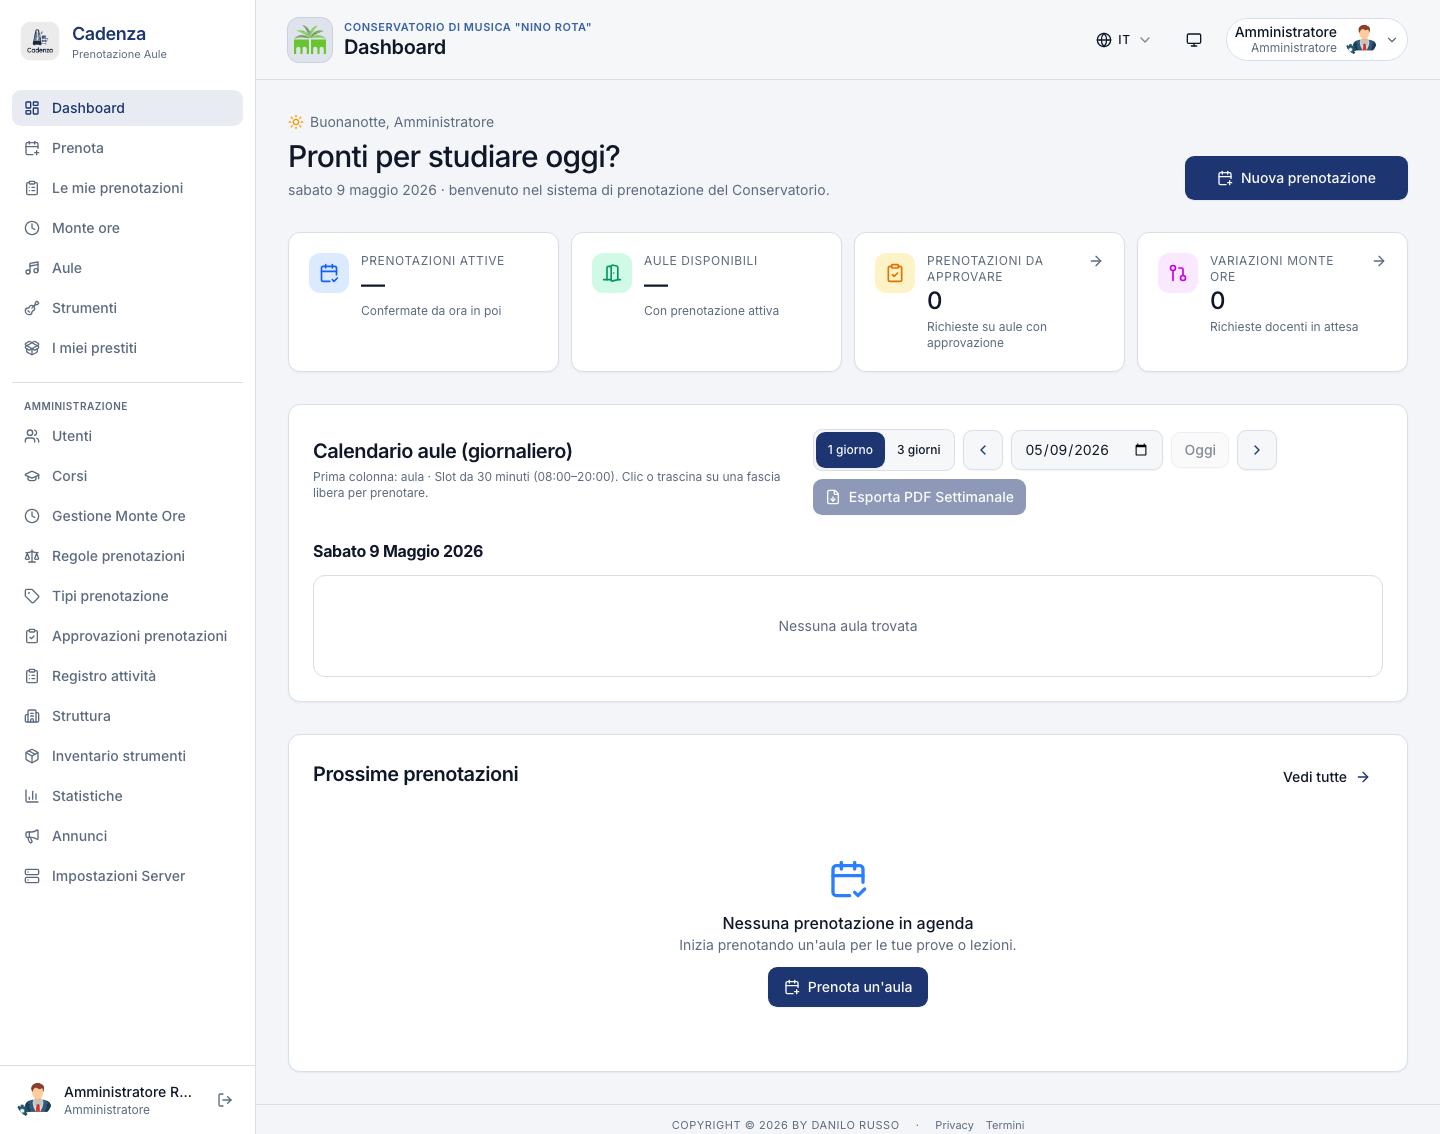
\includegraphics[width=0.95\linewidth]{screenshots/dashboard-overview.png}\caption*{Dashboard — vista calendario "1 giorno" (default)}\end{figure}

Le aule sono in colonna, le ore in riga (slot da 30 min). Colori:

\begin{itemize}
  \item \textcolor{blue!60!white}{$\blacksquare$} \textbf{Blu}: prenotazione tua;
  \item \textcolor{violet}{$\blacksquare$} \textbf{Viola}: prenotazione di un altro utente (non disponibile);
  \item \textcolor{green!50!black}{$\blacksquare$} \textbf{Verde tenue}: slot libero.
\end{itemize}

Click su uno slot libero ti porta direttamente al form di prenotazione, con orario e aula pre-compilati.

\subsection{3.2 Vista 3 giorni}


In alto a destra c'è un toggle "1 giorno · 3 giorni". Cambiandolo vedi tre colonne giorno affiancate, utile per pianificare la settimana o cercare aule libere.

\begin{figure}[H]\centering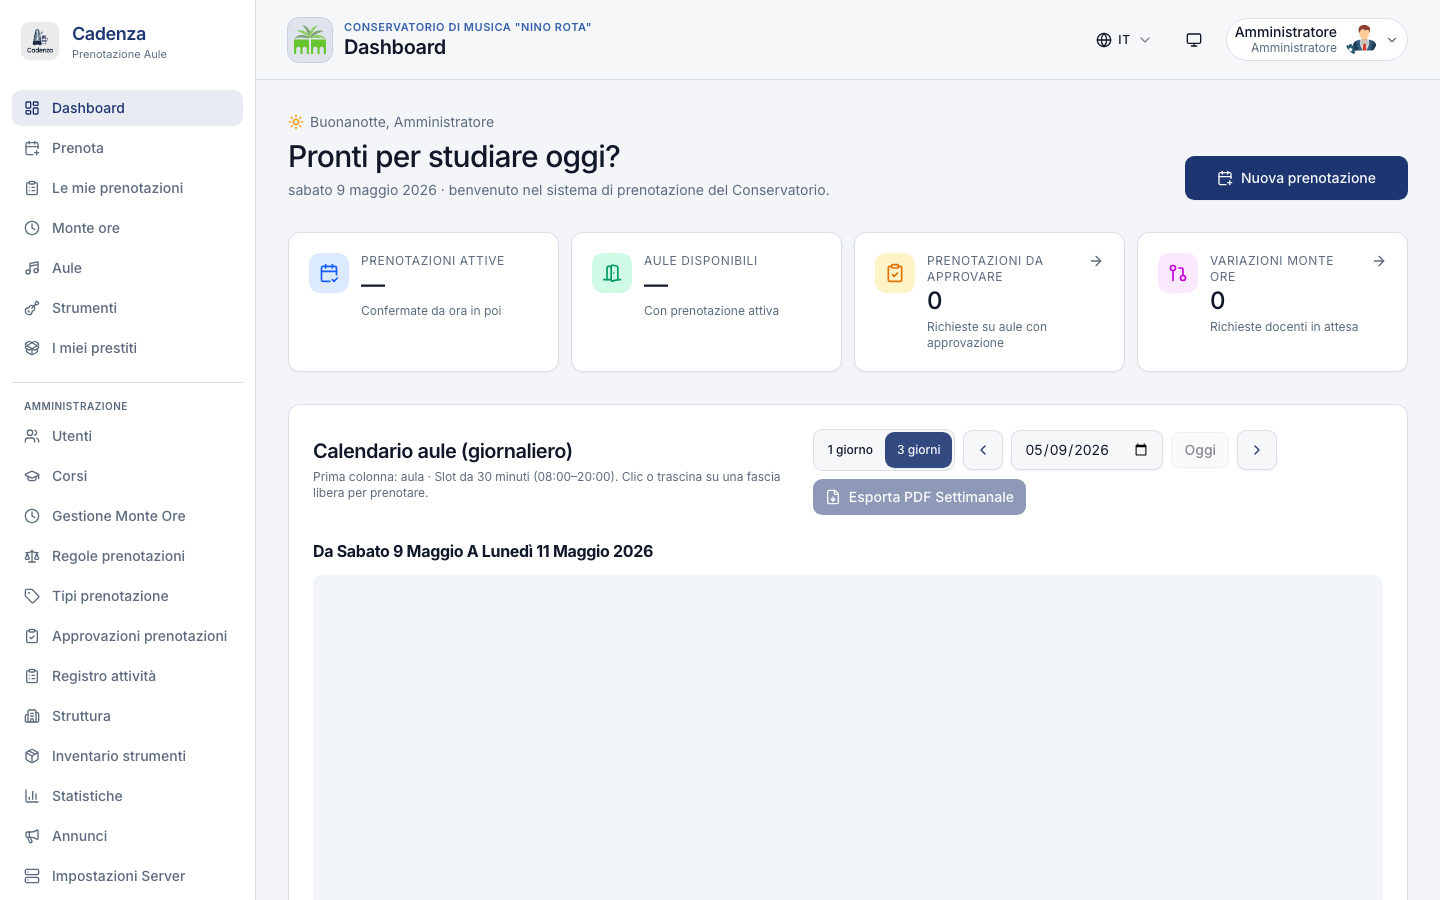
\includegraphics[width=0.95\linewidth]{screenshots/dashboard-calendario-3giorni.png}\caption*{Dashboard — vista calendario "3 giorni" affiancati}\end{figure}

\begin{quote}
La preferenza tra "1 giorno" e "3 giorni" viene \textbf{ricordata sul tuo browser}: la prossima volta che apri Cadenza ritrovi la stessa vista.
\end{quote}

\subsection{3.3 Frecce di navigazione}


Le frecce \texttt{‹} \texttt{›} accanto al titolo del giorno si comportano coerentemente con la vista attiva: in modalità "1 giorno" spostano di un giorno, in modalità "3 giorni" spostano di tre. Il bottone "Oggi" riporta al giorno corrente.

\subsection{3.4 Sidebar}


A sinistra trovi la sidebar con le aree principali:

\begin{itemize}
  \item \textit{[home]} \textbf{Dashboard} (la home)
  \item \textit{[cal]} \textbf{Prenota} --- apre il form di prenotazione completo
  \item \textit{[lista]} \textbf{Le mie prenotazioni} --- il riepilogo storico
  \item  \textbf{Aule} --- la directory degli spazi
  \item  \textbf{Strumenti} --- l'inventario per i prestiti (se attivo)
  \item \textit{[ore]} \textbf{Monte Ore} --- la tua proposta annuale
  \item  \textbf{Avvisi} --- bacheca della Direzione
  \item \textit{[profilo]} \textbf{Profilo} --- anagrafica, password, notifiche, iCal
\end{itemize}

\medskip\hrule\medskip

\section{4. Prenotare un'aula}


URL: \texttt{/booking} (o click sulla cella libera nel calendario, oppure "Prenota" nella sidebar).

\begin{figure}[H]\centering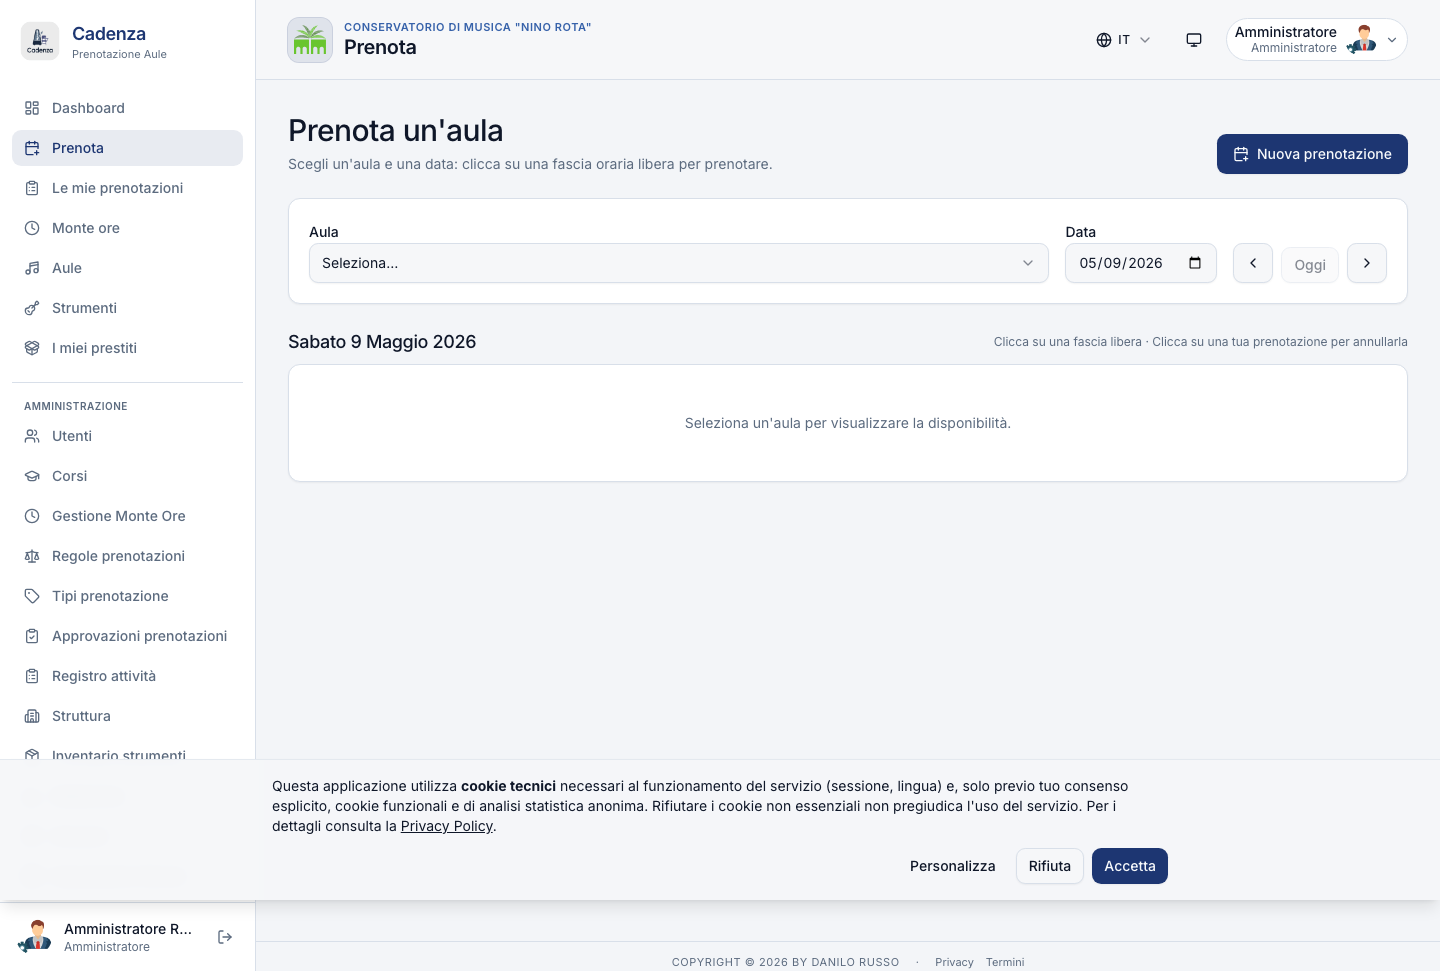
\includegraphics[width=0.95\linewidth]{screenshots/booking-page.png}\caption*{Pagina di prenotazione — selezione aula + slot 30 min}\end{figure}

\subsection{4.1 Il form}


\begin{table}[H]
\centering
\small
\begin{tabularx}{\linewidth}{|X|X|}
\hline
\rowcolor{tableheader} Campo & Cosa fa \\
\hline
\textbf{Aula} & Scegli dal menu raggruppato per edificio. Le aule "non prenotabili" o "non per il tuo ruolo" sono nascoste. \\
\hline
\textbf{Data} & Date picker. Massimo l'anticipo concesso dalla regola del tuo ruolo (default 60 giorni per i docenti). \\
\hline
\textbf{Dalle / Alle} & Slot a 30 minuti. Durata fra il minimo e il massimo previsti per il tuo ruolo (default 30--240 min). \\
\hline
\textbf{Tipo attività} & Lezione · Studio individuale · Prova · Concerto. Influenza alcune quote (es. concerti sono limitati di più). \\
\hline
\textbf{Etichetta} & Testo libero (max 255 caratteri). Es. "Lezione pianoforte 3°". \\
\hline
\textbf{Note} & Eventuali note per la Direzione (facoltativo). \\
\hline
\end{tabularx}
\end{table}


\subsection{4.2 Quando una prenotazione viene rifiutata}


Cadenza controlla, in ordine:

\begin{enumerate}
  \item \textbf{Tu sei attivo e approvato} (lo sei se sei loggato).
  \item L'\textbf{aula è prenotabile} (non disattivata).
  \item \textbf{Non c'è già un'altra prenotazione} sull'aula in quella fascia oraria.
  \item \textbf{Tu non hai già un'altra prenotazione} in un'altra aula nella stessa fascia (un docente non può essere in due posti).
  \item \textbf{Le regole} per il ruolo "docente" (max ore/settimana, durata massima, finestra oraria, cooldown) sono rispettate.
  \item \textbf{Le quote} specifiche (per tipo aula, stanza, edificio) sono rispettate.
  \item Nessuna \textbf{eccezione attiva} copre quella fascia (es. aula in ristrutturazione, festa patronale, sessione esami).
\end{enumerate}

Se uno dei controlli fallisce, vedi un messaggio leggibile in cima al form, tipo:

\begin{quote}
\textit{Hai superato le ore settimanali consentite (30/30). Riprova la prossima settimana.}
\end{quote}

\subsection{4.3 Aule che richiedono approvazione}


Alcune aule (sala concerti, auditorium, sale di rappresentanza) hanno il flag "richiede approvazione" attivo. Quando le prenoti:

\begin{enumerate}
  \item La tua richiesta entra in stato \textbf{"In attesa di approvazione"} (non occupa l'aula).
  \item La Direzione riceve una notifica e decide entro pochi giorni.
  \item Tu ricevi un'email \textbf{approvata} o \textbf{rifiutata con motivo}.
  \item Solo dopo l'approvazione la prenotazione è definitiva e compare nel calendario aule.
\end{enumerate}

\begin{quote}
Le aule che richiedono approvazione mostrano un'icona "\checkmark{}" accanto al nome nel menu di scelta.
\end{quote}

\subsection{4.4 Quick book (template)}


Se prenoti regolarmente la stessa aula nello stesso orario (es. lezione lunedì 14-16 in Aula 12), puoi salvare un \textbf{template} dalla Dashboard. Click su "Salva come template" dopo aver creato una prenotazione, dagli un nome (es. "Lezione lunedì"), e per i prossimi giorni della stessa fascia trovi un bottone "Quick book" che precompila tutto in un click.

\begin{quote}
\textbf{Differenza con il Monte Ore}: il Quick book è per prenotazioni occasionali ricorrenti. Per le \textbf{lezioni annuali} che ripeti ogni settimana per tutto l'anno accademico, usa direttamente il \textbf{Monte Ore} (§8): è pensato apposta.
\end{quote}

\medskip\hrule\medskip

\section{5. Le tue prenotazioni}


URL: \texttt{/my-bookings}

\begin{figure}[H]\centering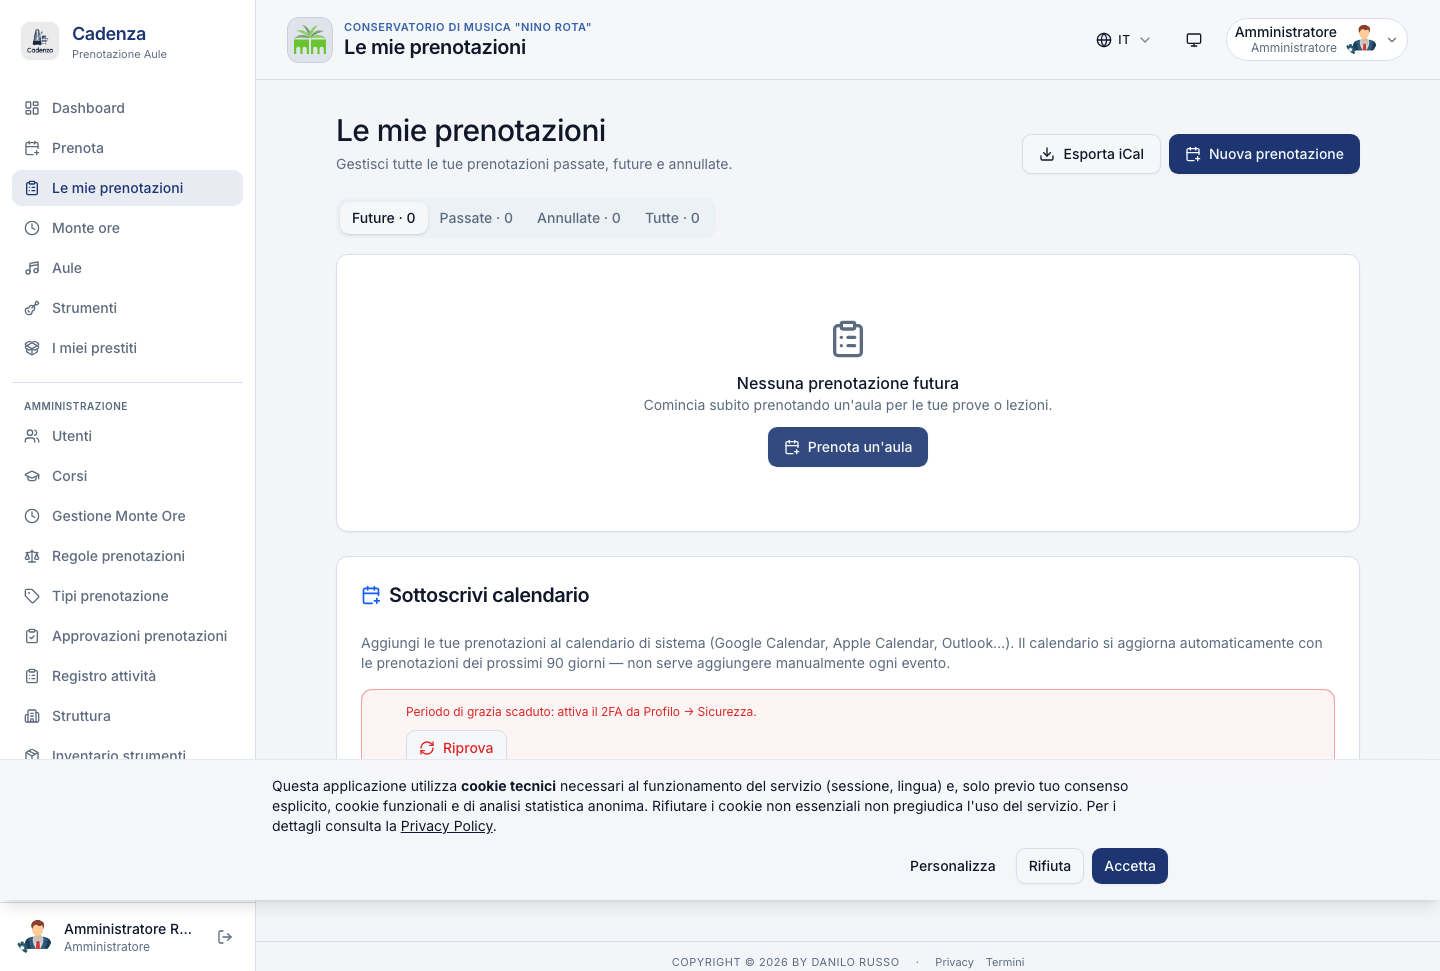
\includegraphics[width=0.95\linewidth]{screenshots/my-bookings.png}\caption*{Le mie prenotazioni — tab future, passate, annullate}\end{figure}

Tre tab:

\begin{table}[H]
\centering
\small
\begin{tabularx}{\linewidth}{|X|X|}
\hline
\rowcolor{tableheader} Tab & Cosa contiene \\
\hline
\textbf{Future} & Prenotazioni confermate (o in attesa di approvazione) dal momento attuale in poi. \\
\hline
\textbf{Passate} & Storico delle prenotazioni concluse. Utile per verificare le ore svolte. \\
\hline
\textbf{Annullate} & Prenotazioni che hai cancellato tu o che la Direzione ha cancellato. \\
\hline
\end{tabularx}
\end{table}


\subsection{5.1 Azioni per ogni prenotazione}


\begin{table}[H]
\centering
\small
\begin{tabularx}{\linewidth}{|X|X|}
\hline
\rowcolor{tableheader} Azione & Quando disponibile \\
\hline
\textbf{\textit{canc.} Cancella} & Sempre, ma se sei sotto il "cancel cutoff" (default 2 ore prima) la cancellazione conta come no-show e impatta le tue statistiche. \\
\hline
\textbf{\textit{mod.} Modifica} & Solo per le prenotazioni future che NON sono già state "checked-in". \\
\hline
\textbf{\textit{[cal]} Aggiungi al calendario} & Scarica un file \texttt{.ics} da importare in Google Calendar, Outlook, Apple Calendar. \\
\hline
\textbf{\textit{[link]} Copia link} & URL diretto alla prenotazione (utile per condividerla con un collega). \\
\hline
\end{tabularx}
\end{table}


\subsection{5.2 Cosa significa "no-show"}


Se hai prenotato un'aula e non hai fatto \textbf{check-in} entro 15 minuti dall'inizio (vedi §6), la prenotazione viene \textbf{automaticamente cancellata} dal sistema, l'aula liberata, e tu accumuli un "no-show" nelle tue statistiche. Tre no-show in un mese tipicamente fanno scattare un avviso dal coordinatore.

\medskip\hrule\medskip

\section{6. Check-in con QR code}


\begin{quote}
\textbf{Cos'è}: una "presentazione all'aula" che conferma che ci sei davvero. Il sistema lo richiede per evitare il fenomeno del "ghost booking" (aule prenotate ma vuote, mentre altri non trovano posto).
\end{quote}

\subsection{6.1 Come funziona}


In ogni aula prenotabile c'è un \textbf{foglio A4} appeso vicino alla porta, con il QR code dell'aula:

\begin{lstlisting}
        ╔══════════════════════╗
        ║  Aula 12 · Storico   ║
        ║                      ║
        ║  ┌──────────────┐    ║
        ║  │              │    ║
        ║  │   QR CODE    │    ║
        ║  │              │    ║
        ║  └──────────────┘    ║
        ║                      ║
        ║  Inquadra con la     ║
        ║  fotocamera del tel  ║
        ╚══════════════════════╝
\end{lstlisting}

\begin{enumerate}
  \item Arrivi in aula 5 minuti prima dell'orario di prenotazione.
  \item Apri la fotocamera del telefono e inquadri il QR.
  \item Si apre Cadenza con il messaggio "Check-in confermato per Aula 12 alle 14:00".
\end{enumerate}

\begin{quote}
Devi essere \textbf{già loggato} in Cadenza sul telefono perché il check-in funzioni. Se non lo sei, Cadenza ti chiede di farlo (1 click).
\end{quote}

\subsection{6.2 Grace period e auto-cancel}


\begin{itemize}
  \item Puoi fare check-in \textbf{fino a 5 minuti prima} dell'orario (\texttt{CHECKIN\_EARLY\_MINUTES}, configurabile).
  \item Hai \textbf{15 minuti di tolleranza} dopo l'inizio (\texttt{GHOST\_GRACE\_MINUTES}, configurabile).
  \item Oltre, la prenotazione viene \textbf{auto-cancellata} + ti arriva un'email di notifica.
\end{itemize}

\subsection{6.3 Aule senza check-in obbligatorio}


Alcune aule (uffici, sale di rappresentanza, sale prove "fidate") possono avere il check-in \textbf{disattivato} dalla Direzione. In quel caso non c'è nessun foglio QR e nessun auto-cancel: il fatto stesso di aver prenotato basta. Lo riconosci perché in \texttt{/my-bookings} la card della prenotazione mostra un'etichetta "Check-in non richiesto".

\medskip\hrule\medskip

\section{7. Aule e dotazioni}


URL: \texttt{/rooms}

\begin{figure}[H]\centering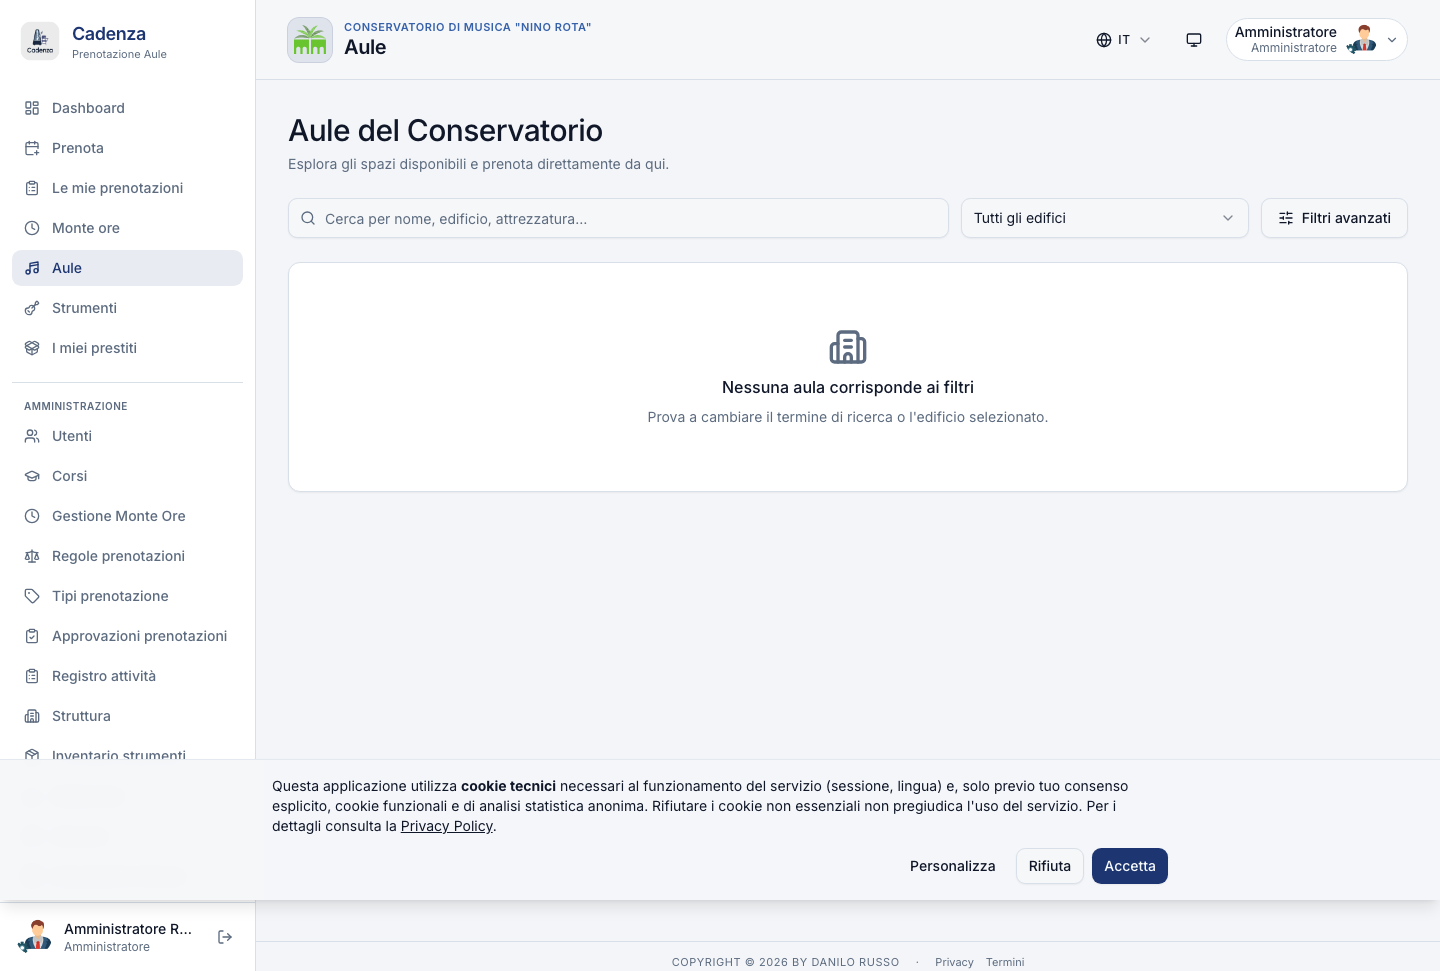
\includegraphics[width=0.95\linewidth]{screenshots/rooms-grouped.png}\caption*{Pagina Aule — sezioni espandibili per edificio}\end{figure}

Directory degli spazi del Conservatorio, \textbf{raggruppata per edificio}:

\begin{itemize}
  \item Ogni edificio è una \textbf{sezione espandibile} con il proprio colore distintivo.
  \item Per ogni aula vedi: nome + codice, capienza, tipologia, dotazioni principali (pianoforte, leggii, mixer, \ldots{}), foto e bottone "Prenota".
  \item Lo stato espanso/collassato di ogni gruppo viene ricordato per la sessione.
\end{itemize}

Usa questa pagina quando:

\begin{itemize}
  \item Vuoi vedere \textbf{quali aule hanno il pianoforte a coda} (filtra per dotazione).
  \item Stai cercando un'aula con una \textbf{capienza specifica} (es. masterclass per 30 persone).
  \item Vuoi controllare la \textbf{foto} di un'aula che non hai mai usato.
\end{itemize}

\begin{quote}
\textbf{Differenza con la Dashboard}: la Dashboard mostra \textbf{chi sta usando} le aule \textbf{adesso}. La pagina Aule mostra \textbf{com'è fatta} ogni aula a prescindere dall'occupazione.
\end{quote}

\medskip\hrule\medskip

\section{8. Monte Ore --- il piano annuale}


URL: \texttt{/monte-ore}

\begin{quote}
\textbf{Cos'è il Monte Ore}: è il \textbf{piano annuale di insegnamento}. Contrattualmente devi garantire almeno \textbf{324 ore di didattica} all'anno (se sei titolare), distribuite in \textbf{2-4 giorni a settimana}, nella finestra di lezioni stabilita dalla Direzione (di solito ott $\rightarrow$ giu). Per chi ha contratto orario, la soglia è personalizzata (tipicamente 30-200 h).
\end{quote}

\subsection{8.1 Quando compilare la proposta}


La Direzione apre una \textbf{finestra di inserimento} ogni anno (es. 15 set -- 15 ott). Vedrai un avviso nella Dashboard. Dentro la finestra puoi:

\begin{itemize}
  \item Creare il tuo pattern settimanale
  \item Modificarlo quante volte vuoi
  \item Inviare la proposta al coordinatore quando sei pronto
\end{itemize}

Fuori dalla finestra l'invio è bloccato (a meno che la Direzione ti abbia concesso una \textbf{deroga individuale} --- vedi §8.10).

\subsection{8.2 Le due sezioni della pagina}


La pagina \texttt{/monte-ore} ha due sezioni in cascata:

\begin{enumerate}
  \item \textbf{Sezione A --- Pattern settimanale}: definisci le tue "fasce ricorrenti" (es. "Lun 14-17 in Aula 12, Mer 14-17 in Aula 12, Ven 9-12 in Aula 5"). Sono i mattoni della tua settimana tipo.
  \item \textbf{Sezione B --- Griglia annuale}: il pattern viene espanso su tutte le settimane dell'anno accademico (al netto delle vacanze). Sulla griglia puoi accendere o spegnere singole celle per personalizzare.
\end{enumerate}

\subsection{8.3 Compilare il pattern settimanale (Sezione A)}


Click su \textbf{+ Aggiungi fascia}. Si apre un dialog con:

\begin{table}[H]
\centering
\small
\begin{tabularx}{\linewidth}{|X|X|}
\hline
\rowcolor{tableheader} Campo & Cosa metti \\
\hline
\textbf{Giorno della settimana} & Lun · Mar · Mer · Gio · Ven · Sab \\
\hline
\textbf{Inizio / Fine} & Orari a granulazione 30 min \\
\hline
\textbf{Aula preferita} & Scegli un'aula dal menu (oppure lascia "qualunque" --- il coordinatore assegnerà) \\
\hline
\textbf{Tipo attività} & Lezione · Studio individuale · Prova · Concerto \\
\hline
\textbf{Etichetta} & Testo libero (es. "Pianoforte 3°", "Solfeggio biennio") \\
\hline
\end{tabularx}
\end{table}


Aggiungi tutte le fasce della tua settimana. Le vedi in tabella sotto:

\begin{lstlisting}
  Giorno    Orario      Aula                 Tipo       Etichetta
  ─────     ───────     ─────────────────    ────────   ─────────────
  Lun       14:00–17:00 Aula 12 · Storico    Lezione    Pianoforte 3°
  Mer       14:00–17:00 Aula 12 · Storico    Lezione    Pianoforte 3°
  Ven       09:00–12:00 Aula 5 · Storico     Lezione    Pianoforte 1°
\end{lstlisting}

\textbf{Regole CCNL}:

\begin{itemize}
  \item Minimo \textbf{2 giorni diversi} della settimana, massimo \textbf{4}. Se metti 5 giorni il sistema te lo segnala come errore.
  \item La somma delle ore della settimana × numero di settimane dell'anno deve essere \textbf{$\geq$ alla tua soglia annua} (324 h se sei titolare, altrimenti la tua soglia personalizzata).
\end{itemize}

Cadenza ti aiuta mostrando in alto \textbf{Totale ore proposte / Soglia annua} in tempo reale:

\begin{itemize}
  \item \textcolor{green!60!black}{$\bullet$} Verde se sei $\geq$ soglia $\rightarrow$ puoi inviare
  \item \textcolor{yellow!70!black}{$\bullet$} Ambra se sei sotto soglia $\rightarrow$ completa prima di inviare
\end{itemize}

\subsection{8.4 La griglia annuale (Sezione B)}


Una volta che il pattern è compilato, click su \textbf{"Rigenera dalla Sezione A"}. Il sistema espande il pattern su tutte le settimane lavorative dell'anno, escludendo automaticamente le vacanze e le festività infrasettimanali configurate dalla Direzione.

La griglia mostra \textbf{settimana × giorno}, con le celle colorate:

\begin{itemize}
  \item \textcolor{blue!60!white}{$\blacksquare$} \textbf{Blu}: cella attiva (la userai per fare lezione)
  \item \textcolor{black!30}{$\square$} \textbf{Vuota}: cella inattiva (puoi cliccarla per attivarla)
  \item \textcolor{red}{$\blacksquare$} \textbf{Rossa}: cella bloccata (festività, vacanze --- non cliccabile)
\end{itemize}

Click su una cella attiva $\rightarrow$ la disattivi (libera quelle ore).   Click su una cella vuota $\rightarrow$ la attivi (la includi nella proposta).

\begin{quote}
Tutte le celle nascono \textbf{inattive} dopo la rigenerazione: tu le accendi cliccando, e il totale ore si aggiorna in tempo reale. Questo ti permette di "saltare" specifiche settimane (es. trasferte, conferenze, scambi Erasmus).
\end{quote}

\subsection{8.5 Soglia ore personalizzata}


Se hai un contratto diverso dal titolare CCNL (contratto orario, supplente part-time, accompagnatore concertistico, ecc.), la Direzione può averti impostato una \textbf{soglia individuale}. In quel caso vedi un banner azzurro in cima:

\begin{figure}[H]\centering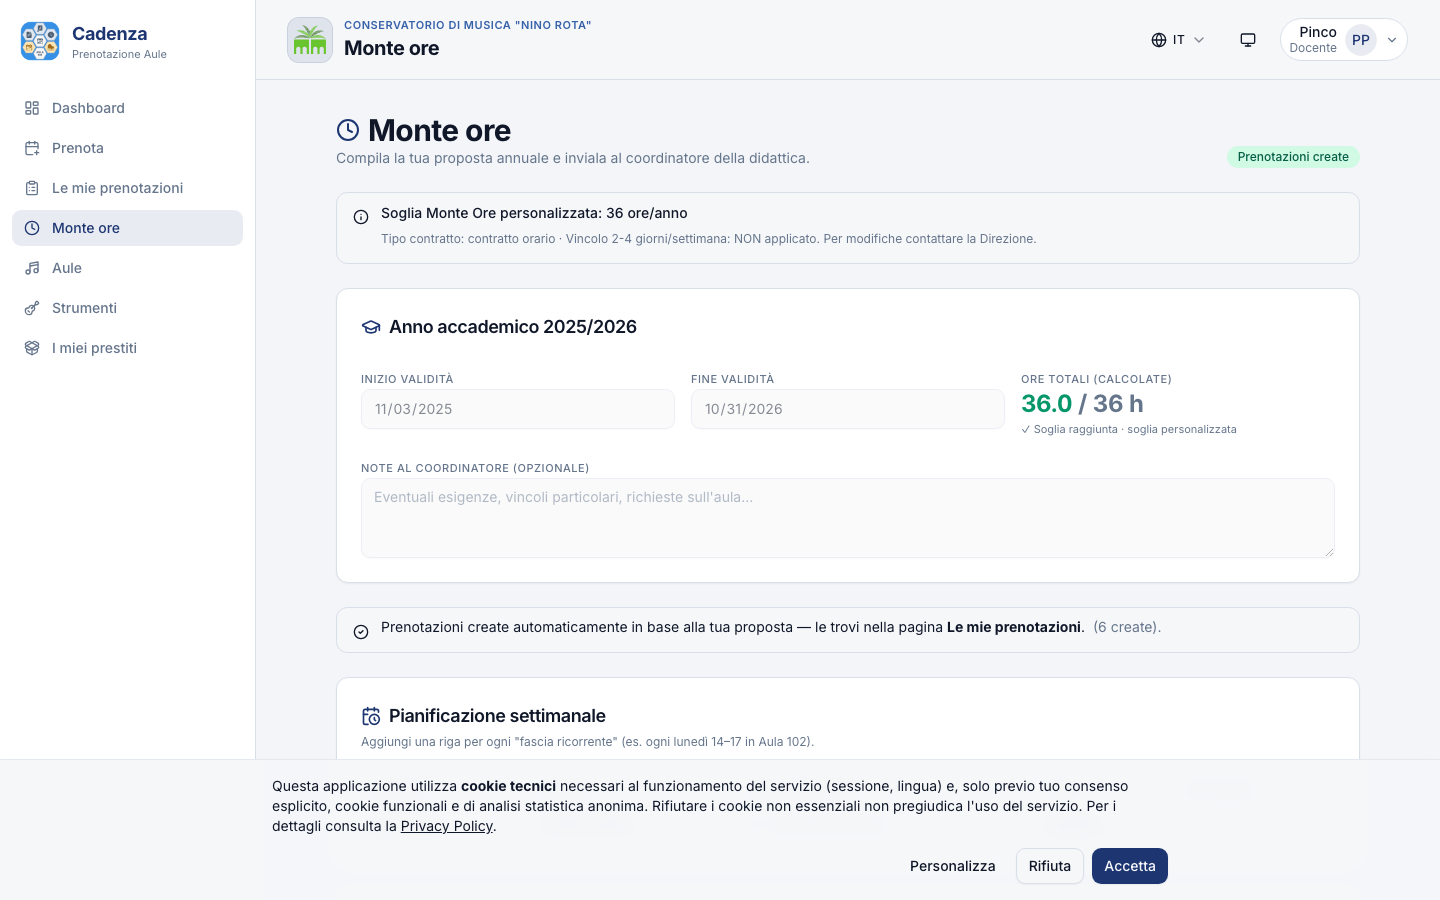
\includegraphics[width=0.95\linewidth]{screenshots/monteore-docente-banner.png}\caption*{Banner deroga Monte Ore personalizzata}\end{figure}

\begin{table}[H]
\centering
\small
\begin{tabularx}{\linewidth}{|X|X|X|}
\hline
\rowcolor{tableheader} Esempio di deroga & Soglia & Bypass vincolo 2-4 gg \\
\hline
Titolare ridotto L.104/92 al 50\% & 162 h & No \\
\hline
Contratto orario 60 h & 60 h & Sì (puoi concentrare tutto in 1 giorno) \\
\hline
Laboratorio musica d'insieme & 120 h & No \\
\hline
Accompagnatore concertistico & 30 h & Sì \\
\hline
\end{tabularx}
\end{table}


\begin{quote}
Per modificare la deroga, contatta la Direzione: tu \textbf{non puoi} cambiarla autonomamente. Le modifiche vengono tracciate in audit log.
\end{quote}

\subsection{8.6 Inviare la proposta}


Quando hai compilato pattern + griglia e il totale ore raggiunge la soglia, click \textbf{"Invia al coordinatore"} in alto a destra.

Il sistema controlla un'ultima volta:

\begin{itemize}
  \item Almeno 2 fasce orarie nel pattern;
  \item Giorni distinti fra 2 e 4 (a meno della tua eventuale deroga);
  \item Totale ore $\geq$ soglia.
\end{itemize}

Se manca qualcosa, vedi un \textbf{Alert} che ti elenca cosa correggere prima di inviare. Il bottone "Invia" è disabilitato finché tutto è verde.

Dopo l'invio la proposta passa in stato \textbf{"In attesa di approvazione"} e arriva al coordinatore.

\subsection{8.7 Stati della proposta}


\begin{table}[H]
\centering
\small
\begin{tabularx}{\linewidth}{|X|X|}
\hline
\rowcolor{tableheader} Stato & Cosa significa per te \\
\hline
\textbf{Bozza} & Stai compilando. Puoi modificare e salvare quante volte vuoi. Nessuno la vede. \\
\hline
\textbf{In attesa} & L'hai inviata. Aspetti la decisione del coordinatore. NON puoi più modificare. \\
\hline
\textbf{Rifiutata} & Il coordinatore ha rifiutato con un motivo. Torna in bozza, modifica, reinvia. \\
\hline
\textbf{Approvata} & Tutto OK. Il coordinatore può ancora assegnare le aule. Le prenotazioni reali non sono ancora state create. \\
\hline
\textbf{Generata} & Il coordinatore ha cliccato "Crea prenotazioni". Adesso le trovi tutte in \texttt{/my-bookings}. \\
\hline
\end{tabularx}
\end{table}


\begin{quote}
\textbf{Differenza tra "approvata" e "generata"}: la prima è la firma contrattuale ("ok, il piano è valido"); la seconda è la materializzazione operativa ("ho creato 600 prenotazioni nel calendario"). Possono passare alcuni giorni tra le due.
\end{quote}

\subsection{8.8 "Richiesta di modifica" dal coordinatore}


Può capitare che il coordinatore non rifiuti la tua proposta in blocco, ma ti chieda una \textbf{correzione mirata} (es. "manca un'ora rispetto al CCNL", "l'aula 12 il martedì è già occupata, scegline un'altra"). In quel caso la proposta \textbf{torna in bozza} e vedi un banner rosso con il motivo:

\begin{lstlisting}
[!] Proposta da rivalidare
    Manca 1 ora alla soglia: aggiungi una fascia di 30 min × 2 settimane.
\end{lstlisting}

Fai le modifiche richieste e clicca di nuovo "Invia al coordinatore".

\subsection{8.9 Cosa NON puoi fare dopo l'invio}


Una volta inviata la proposta NON puoi più modificare il pattern settimanale o cliccare le celle della griglia, finché il coordinatore non decide. Se ti accorgi di un errore importante:

\begin{enumerate}
  \item Scrivigli/parlagli direttamente.
  \item Lui può rifiutare (torni in bozza, riparti da zero) oppure "richiedere modifica" (torni in bozza ma il tuo lavoro è preservato).
\end{enumerate}

\subsection{8.10 Deroga finestra di inserimento (subentro tardivo)}


Se entri in servizio \textbf{dopo che la finestra di inserimento è chiusa} (es. nomina MIUR di novembre, sostituzione a stagione iniziata), chiedi alla Direzione di concederti una \textbf{deroga individuale}. Loro impostano una \textbf{data limite} entro cui tu puoi inviare. Il sistema te lo permette anche se la finestra generale è ormai chiusa.

\begin{quote}
La deroga è personale e nominale: vale solo per te, non riapre la finestra per gli altri docenti.
\end{quote}

\medskip\hrule\medskip

\section{9. Spostamenti e variazioni dopo l'approvazione}


Una volta che la tua proposta è \textbf{"approvata"} o \textbf{"generata"}, le lezioni sono fisse nel calendario. In corso d'anno è normale aver bisogno di:

\begin{itemize}
  \item Cancellare una lezione (visita medica, congresso, malattia)
  \item Spostare una lezione di orario
  \item Cambiare aula per una sola settimana
  \item Recuperare una lezione in un altro giorno
  \item Aggiungere una lezione fuori pattern (recupero compenso)
\end{itemize}

Cadenza ti dà 5 strumenti diversi. Ogni richiesta è una \textbf{variazione} (in inglese: \textit{amendment}).

\subsection{9.1 Limite annuale di variazioni}


Per evitare che la proposta venga riscritta di settimana in settimana, la Direzione imposta un \textbf{massimo di variazioni all'anno} (default: \textbf{3} per proposta). Quando raggiungi il limite, le richieste successive sono bloccate fino al prossimo anno accademico (a meno di intervento manuale dell'admin).

\begin{table}[H]
\centering
\small
\begin{tabularx}{\linewidth}{|X|X|}
\hline
\rowcolor{tableheader} Tipo di variazione & Consuma una variazione? \\
\hline
Disattivazione di una cella & \textbf{No} (libera ore, sempre lecita) \\
\hline
Riattivazione & Sì \\
\hline
Cambio orario & Sì \\
\hline
Cambio aula puntuale & Sì \\
\hline
Spostamento (off+on) & Sì (\textbf{1 sola} variazione, non 2) \\
\hline
Nuovo giorno fuori pattern & Sì \\
\hline
\end{tabularx}
\end{table}


\subsection{9.2 Le 5 azioni di variazione}


\subsubsection{9.2.1 Disattivare una lezione (toggle off)}


\begin{quote}
\textit{"Cancella la lezione del 12 ottobre, sono in trasferta."}
\end{quote}

Dalla griglia annuale, click sulla cella attiva del 12/10. Diventa vuota. La prenotazione corrispondente nel calendario aule si cancella automaticamente. \textbf{Auto-approvata sempre}.

\subsubsection{9.2.2 Riattivare una lezione}


\begin{quote}
\textit{"La lezione del 12 ottobre che avevo cancellato la voglio rimettere."}
\end{quote}

Click sulla cella vuota del 12/10 (sotto un giorno del pattern). Cadenza ricrea la prenotazione, \textbf{auto-approvata} se l'aula è ancora libera.

\subsubsection{9.2.3 Cambiare orario di una sola occorrenza}


\begin{quote}
\textit{"Lunedì 6 novembre ho una visita medica alle 14: inizio alle 16 invece che alle 14."}
\end{quote}

Sulla cella attiva del 6/11, click sulla piccola icona "\textbf{\textbf{:}}" in alto a destra $\rightarrow$ si apre il dialog "Spostamento lezione" $\rightarrow$ tab \textbf{"Cambia orario"} $\rightarrow$ inserisci i nuovi orari (es. 16:00--19:00) $\rightarrow$ "Salva".

\begin{itemize}
  \item \textbf{Auto-approvata} se la cella era nel piano originale.
  \item Tutte le altre lezioni del pattern restano invariate.
  \item La prenotazione nel calendario aule si aggiorna ai nuovi orari.
\end{itemize}

\subsubsection{9.2.4 Cambiare aula puntualmente}


\begin{quote}
\textit{"Mercoledì 8 novembre l'Aula 12 è occupata per un concerto: sposto solo quel mercoledì in Aula 5."}
\end{quote}

Cella attiva del 8/11 $\rightarrow$ icona "\textbf{\textbf{:}}" $\rightarrow$ tab \textbf{"Cambia aula"} $\rightarrow$ seleziona "Aula 5" $\rightarrow$ "Richiedi cambio aula".

\begin{itemize}
  \item \textbf{Sempre pending}: l'aula è risorsa condivisa, il coordinatore deve confermare che Aula 5 è davvero libera.
  \item Quando il coordinatore approva, lo slot del 8/11 prende Aula 5 come aula. Il pattern e tutte le altre settimane restano in Aula 12.
\end{itemize}

\subsubsection{9.2.5 Spostare una lezione su un altro giorno}


\begin{quote}
\textit{"La lezione di lunedì 13 novembre la sposto a giovedì 16 novembre."}
\end{quote}

Cella attiva del 13/11 $\rightarrow$ icona "\textbf{\textbf{:}}" $\rightarrow$ tab \textbf{"Sposta a\ldots{}"} $\rightarrow$ scegli "16/11 14:00--17:00" dall'elenco delle celle libere $\rightarrow$ "Sposta".

\begin{itemize}
  \item \textbf{Auto-approvata} se sia la cella sorgente sia quella destinazione sono già nel tuo pattern settimanale.
  \item \textbf{Pending} se la destinazione è fuori pattern.
  \item Conta come \textbf{1 sola} variazione (non 2): la disattivazione del 13/11 e l'attivazione del 16/11 sono fatte in un'unica operazione atomica.
\end{itemize}

\subsubsection{9.2.6 Aggiungere un giorno fuori pattern}


\begin{quote}
\textit{"Voglio aggiungere una lezione il sabato 18 novembre per recuperare il programma."}
\end{quote}

Pulsante \textbf{"Richiedi nuovo giorno"} in cima alla griglia. Si apre un dialog con:

\begin{table}[H]
\centering
\small
\begin{tabularx}{\linewidth}{|X|X|}
\hline
\rowcolor{tableheader} Campo & Cosa metti \\
\hline
Data & 2026-11-18 \\
\hline
Inizio -- Fine & 09:00 -- 12:00 \\
\hline
Aula preferita & (facoltativa: il coordinatore la assegna) \\
\hline
Tipo & Lezione · Studio · Prova \\
\hline
Etichetta & "Recupero programma 3°" \\
\hline
Note & "Mi mancano 3 ore prima dell'esame" \\
\hline
\end{tabularx}
\end{table}


\begin{itemize}
  \item \textbf{Sempre pending}: il coordinatore deve verificare aula + opportunità.
  \item Quando approvato, viene creato uno slot "fuori pattern" + la prenotazione corrispondente.
\end{itemize}

\subsection{9.3 Dove vedere lo storico delle tue variazioni}


Sotto la griglia annuale c'è una card collassabile \textbf{"Storico variazioni"} con il conteggio:

\begin{itemize}
  \item \textbf{In attesa}: le pending in attesa di decisione del coordinatore
  \item \textbf{Auto-approvate}: quelle che il sistema ha applicato automaticamente
  \item \textbf{Approvate}: le pending che il coordinatore ha approvato
  \item \textbf{Rifiutate}: quelle che il coordinatore ha rifiutato (con motivo visibile)
\end{itemize}

\subsection{9.4 Banner "proposta da rivalidare" in corso d'anno}


Se la Direzione \textbf{modifica il tuo contratto} (es. passi da titolare a titolare ridotto, o ti aggiunge ore per supplenza) \textbf{mentre la tua proposta è già attiva}, Cadenza ti mostra in cima alla pagina Monte Ore un banner rosso:

\begin{lstlisting}
[!] Proposta da rivalidare
    Variazione contratto (admin) in corso d'anno: rivedi e re-invia la proposta.
\end{lstlisting}

Cosa fare:

\begin{enumerate}
  \item Apri la pagina Monte Ore e leggi il motivo del banner.
  \item Verifica il pattern: con la nuova soglia ore, devi aggiungerne / toglierne?
  \item Se serve, aggiungi o rimuovi fasce dal pattern e ri-clicca "Invia al coordinatore".
  \item Il banner sparisce alla prossima submit.
\end{enumerate}

\begin{quote}
Il banner è informativo, \textbf{non blocca} la didattica corrente. Le lezioni continuano regolarmente fino a quando non re-invii.
\end{quote}

\medskip\hrule\medskip

\section{10. Prestiti strumenti}


URL: \texttt{/instruments} (se il modulo è abilitato dalla Direzione)

\begin{figure}[H]\centering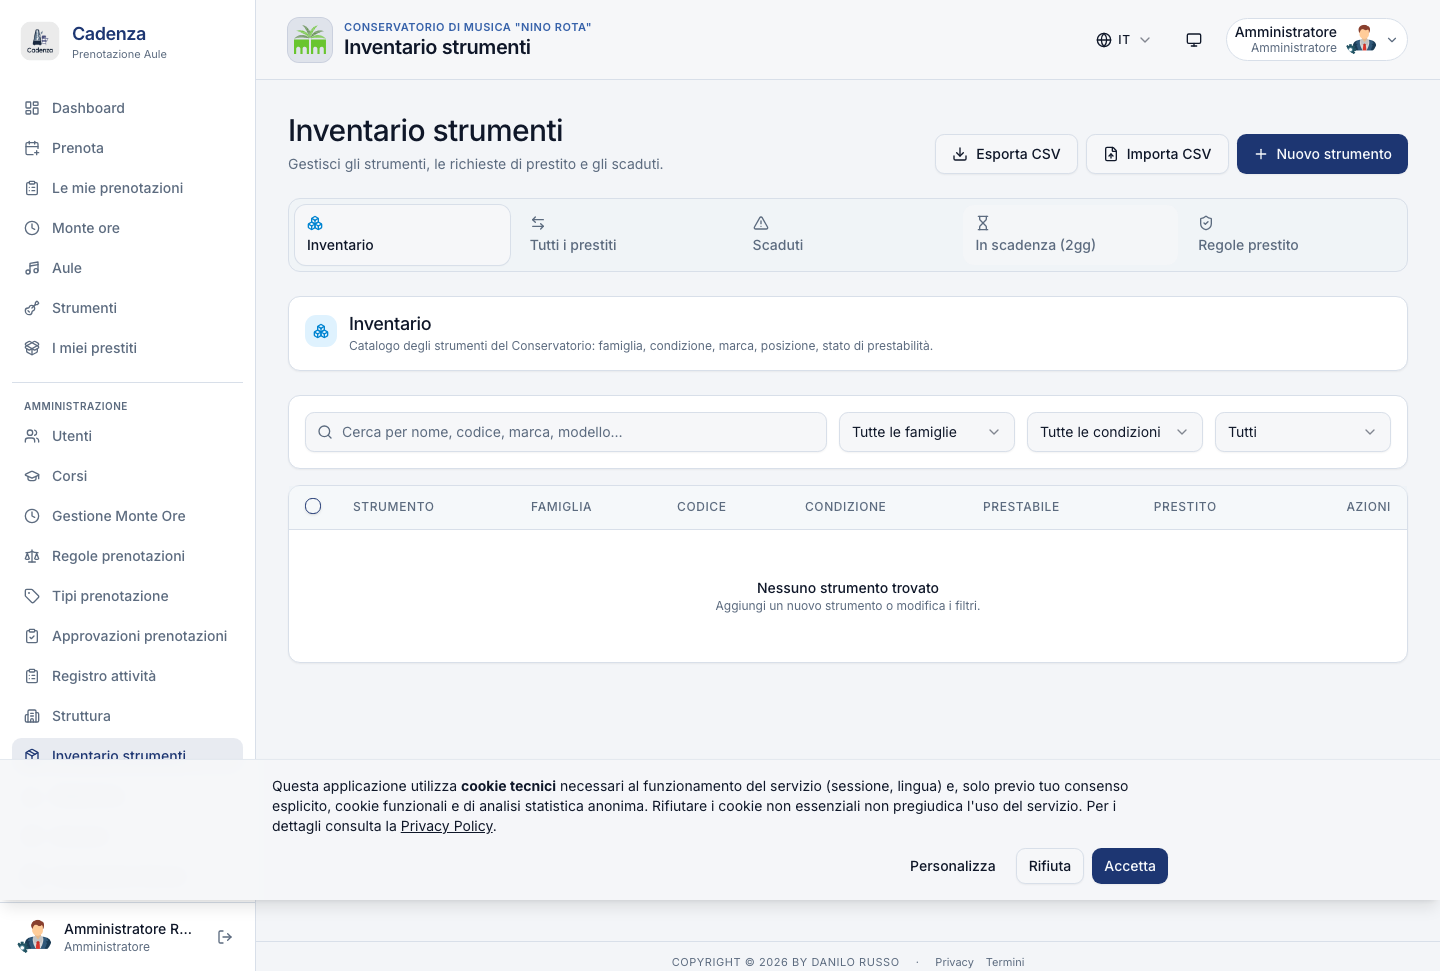
\includegraphics[width=0.95\linewidth]{screenshots/instruments-overview.png}\caption*{Inventario strumenti — vista catalogo}\end{figure}

Cadenza ti permette di richiedere in prestito strumenti dell'inventario del Conservatorio (violini, fiati, percussioni, attrezzature elettroniche, ecc.).

\subsection{10.1 Richiedere un prestito}


\begin{enumerate}
  \item Apri \texttt{/instruments}, filtra per \textbf{famiglia} (archi · fiati · tastiere · \ldots{}) e per \textbf{condizione} (ottimo · buono · \ldots{}).
  \item Clicca sullo strumento che ti serve.
  \item Compila il form prestito: periodo (dal / al), motivo (lezione, prova, evento esterno), note.
  \item Conferma. La richiesta entra in stato \textbf{"richiesto"}.
  \item La Direzione approva (o rifiuta con motivo).
  \item Vai in \texttt{/my-loans} per vedere lo stato.
\end{enumerate}

\subsection{10.2 Quote di prestito}


A seconda del tuo ruolo e della famiglia dello strumento, ci sono \textbf{quote}: numero massimo di prestiti contemporanei e/o giorni cumulati all'anno. Le quote sono visibili nella card di ogni strumento ("max 1 prestito di archi per docente"). Se chiedi un prestito oltre quota, vedi un messaggio chiaro.

\subsection{10.3 PDF di consegna e restituzione}


Quando la Direzione approva, ti arriva via email un \textbf{PDF di consegna} da stampare e firmare. Lo porti al magazziniere il giorno del ritiro; lui ti consegna lo strumento.

Al rientro, idem: il magazziniere genera un \textbf{PDF di restituzione} (firmato anche da te) e chiude il prestito su Cadenza.

\subsection{10.4 Promemoria e ritardi}


\begin{itemize}
  \item \textbf{2 giorni prima} della data di restituzione, ricevi un'email di promemoria.
  \item Se non restituisci entro la data prevista, il prestito passa in stato \textbf{"scaduto"} e ricevi un'email ogni 7 giorni finché non chiudi.
  \item Tre prestiti scaduti accumulati possono comportare la sospensione della quota fino a fine anno (politica della Direzione).
\end{itemize}

\medskip\hrule\medskip

\section{11. Avvisi e bacheca}


URL: \texttt{/announcements}

\begin{figure}[H]\centering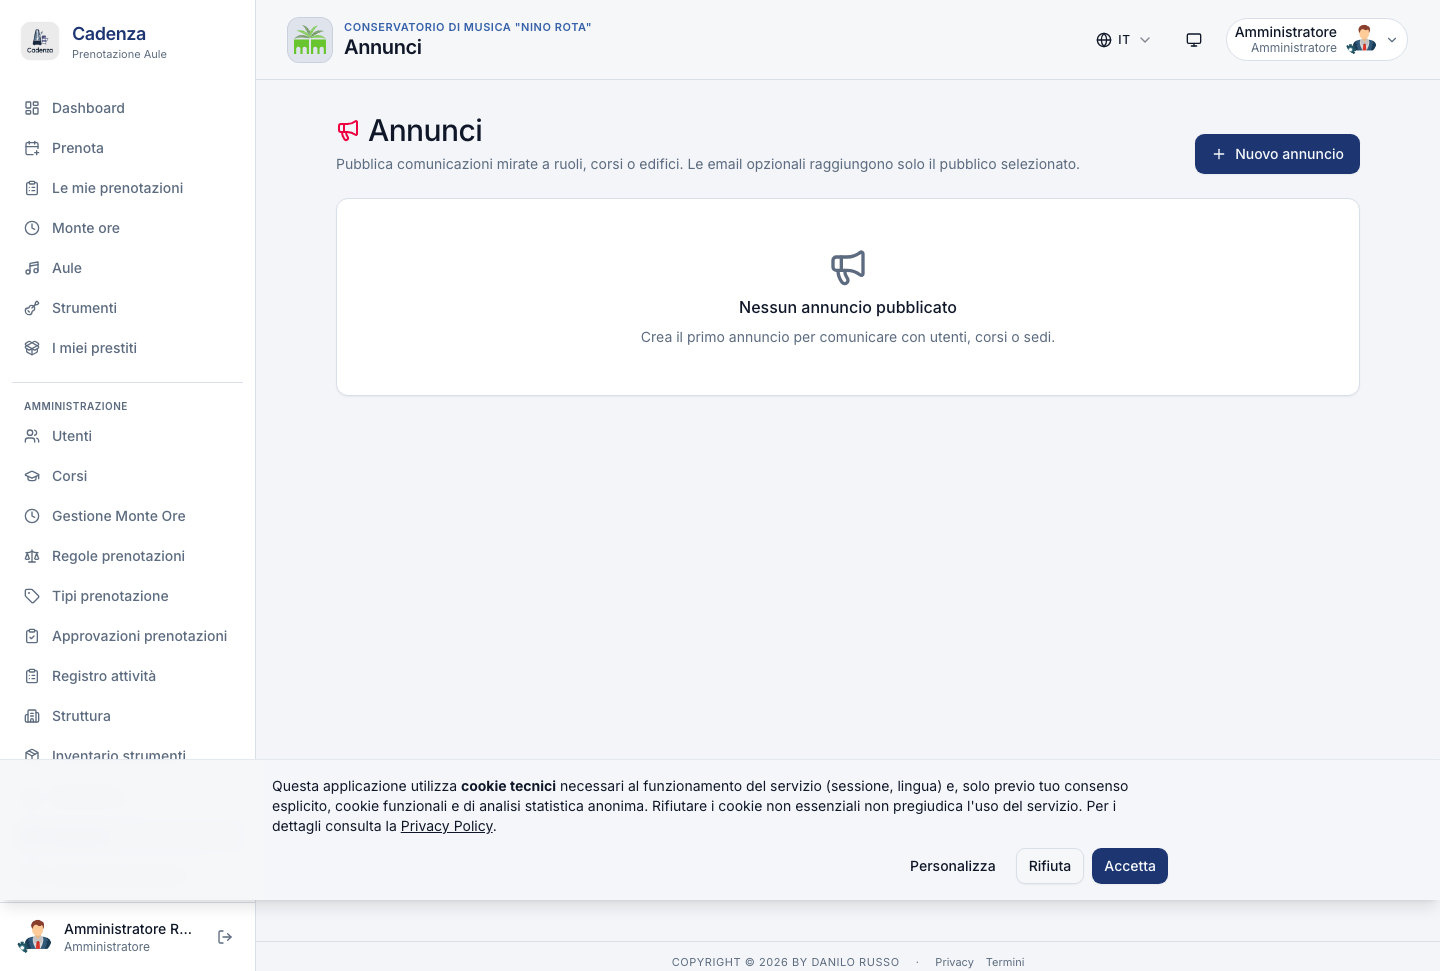
\includegraphics[width=0.95\linewidth]{screenshots/announcements-overview.png}\caption*{Bacheca avvisi — griglia di card con badge audience}\end{figure}

Gli avvisi sono pubblicati dalla Direzione, filtrati per \textbf{audience}:

\begin{itemize}
  \item A tutti
  \item Per ruolo (solo docenti)
  \item Per corso (es. solo Pianoforte)
  \item Per edificio (es. solo Sede succursale)
\end{itemize}

Vedi solo gli avvisi che riguardano te. Ogni card mostra titolo, corpo (markdown semplice), data di pubblicazione, scadenza, badge "Pinnato" se importante.

\begin{quote}
Gli avvisi importanti compaiono anche \textbf{in cima alla Dashboard} la prima volta che entri. Se li chiudi con la X, restano comunque sulla pagina \texttt{/announcements} finché non scadono.
\end{quote}

\medskip\hrule\medskip

\section{12. Profilo, notifiche e calendario personale}


URL: \texttt{/profile}

\begin{figure}[H]\centering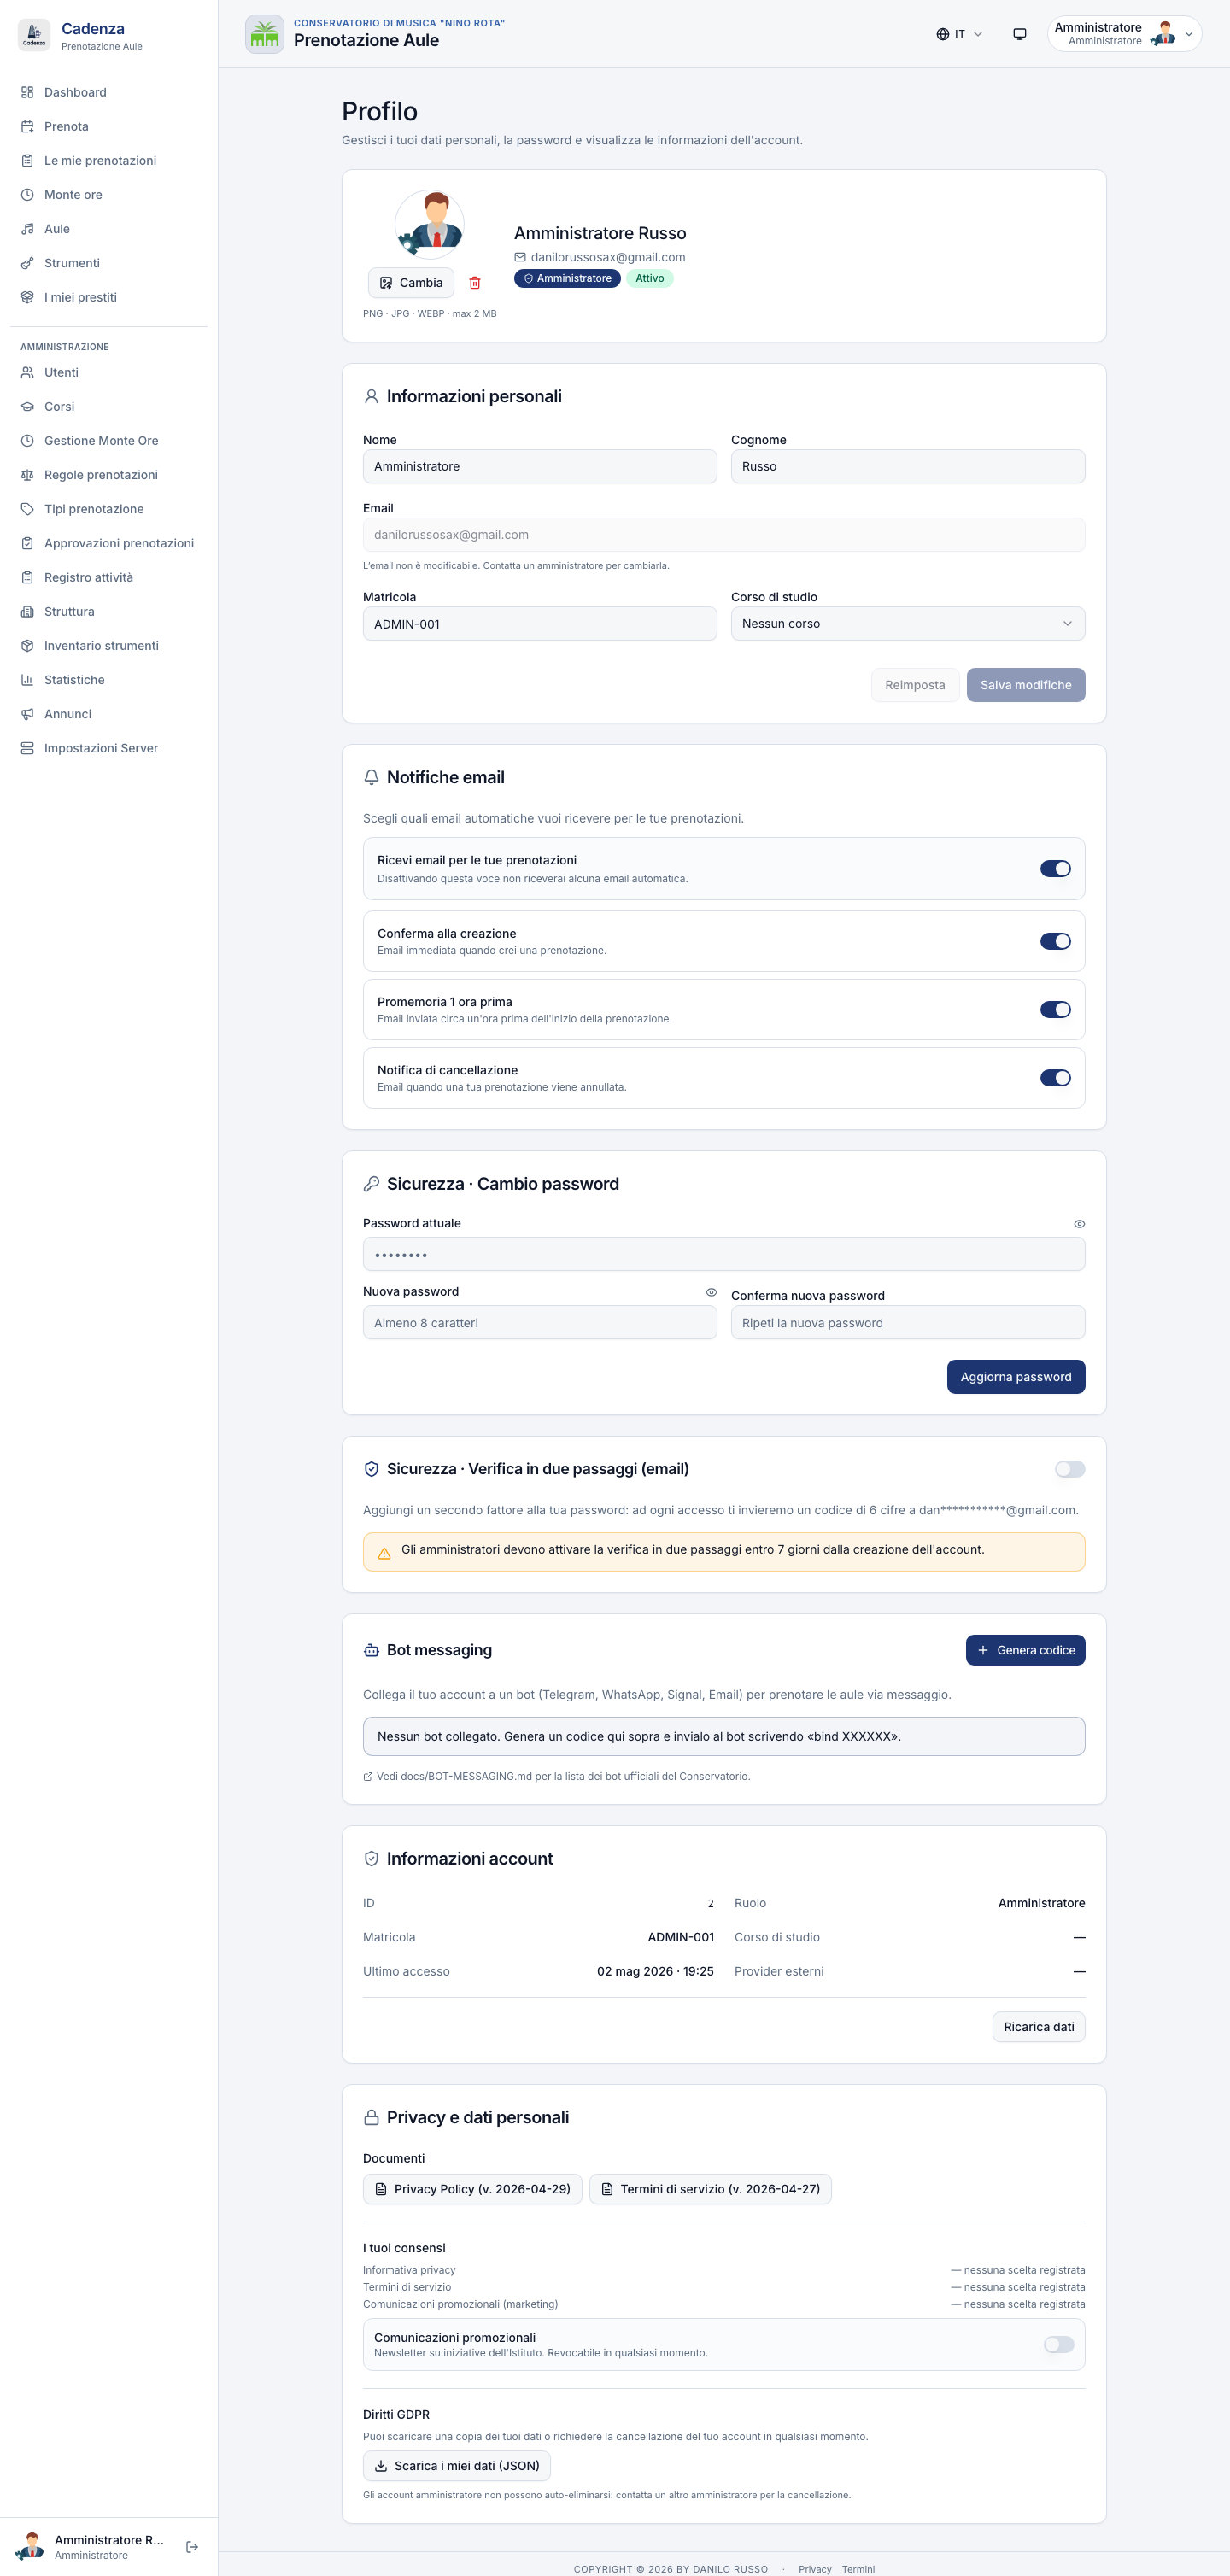
\includegraphics[width=0.95\linewidth]{screenshots/profile-page.png}\caption*{Pagina Profilo — anagrafica e preferenze}\end{figure}

\subsection{12.1 Anagrafica}


Aggiorna nome, cognome, matricola, corso (se applicabile). L'email non si cambia direttamente: contatta la Segreteria.

\subsection{12.2 Password}


Cambia la password. La nuova deve avere \textbf{almeno 10 caratteri}, una \textbf{maiuscola} e una \textbf{cifra} (linee guida AGID 2024).

\subsection{12.3 Preferenze notifiche email}


Tre interruttori indipendenti:

\begin{table}[H]
\centering
\small
\begin{tabularx}{\linewidth}{|X|X|}
\hline
\rowcolor{tableheader} Notifica & Quando ti arriva \\
\hline
\textbf{Conferma prenotazione} & Subito dopo aver salvato una nuova prenotazione. \\
\hline
\textbf{Promemoria} & 24 h prima dell'orario di una prenotazione. \\
\hline
\textbf{Cancellazione} & Quando una prenotazione viene cancellata (da te, da admin, o auto-cancel ghost). \\
\hline
\end{tabularx}
\end{table}


Default: tutti e tre attivi. Disattivali se preferisci notifiche minimali.

\subsection{12.4 Token iCal (calendario personale)}


Cadenza pubblica un \textbf{calendario iCal personale} con tutte le tue prenotazioni. Per usarlo:

\begin{enumerate}
  \item Click su \textbf{"Mostra link iCal"} nella card "Sincronizza calendario".
  \item Copia l'URL (formato \texttt{https://cadenza.example.it/api/users/me/ical/\textless{}token\textgreater{}}).
  \item Importalo nel tuo client preferito (Apple Calendar, Google Calendar, Outlook).
  \item Da quel momento, ogni nuova prenotazione/cancellazione si sincronizza automaticamente.
\end{enumerate}

\begin{quote}
Il token è \textbf{segreto}: non condividerlo. Se lo rigeneri (bottone "Rigenera token") il vecchio smette di funzionare e dovrai aggiornare il client.
\end{quote}

\subsection{12.5 Cancella account (art. 17 GDPR)}


In coda alla pagina c'è un bottone rosso \textbf{"Richiedi cancellazione account"}. Compila la motivazione (es. "Pensionamento") $\rightarrow$ la Direzione riceve la richiesta e procede. I dati vengono cancellati nei tempi previsti dal GDPR (di norma 30 giorni).

\subsection{12.6 Esporta dati (art. 20 GDPR)}


Bottone \textbf{"Esporta i miei dati"} $\rightarrow$ scarichi un file ZIP con tutto quello che Cadenza ha su di te: prenotazioni, monte ore, prestiti, audit log, consensi cookie. Utile per portabilità verso un altro sistema, o per archivio personale.

\medskip\hrule\medskip

\section{13. App sul telefono (PWA)}


Cadenza è una \textbf{PWA} (Progressive Web App): puoi installarla sul telefono come fosse un'app nativa, \textbf{senza passare da Google Play o App Store}.

\begin{figure}[H]\centering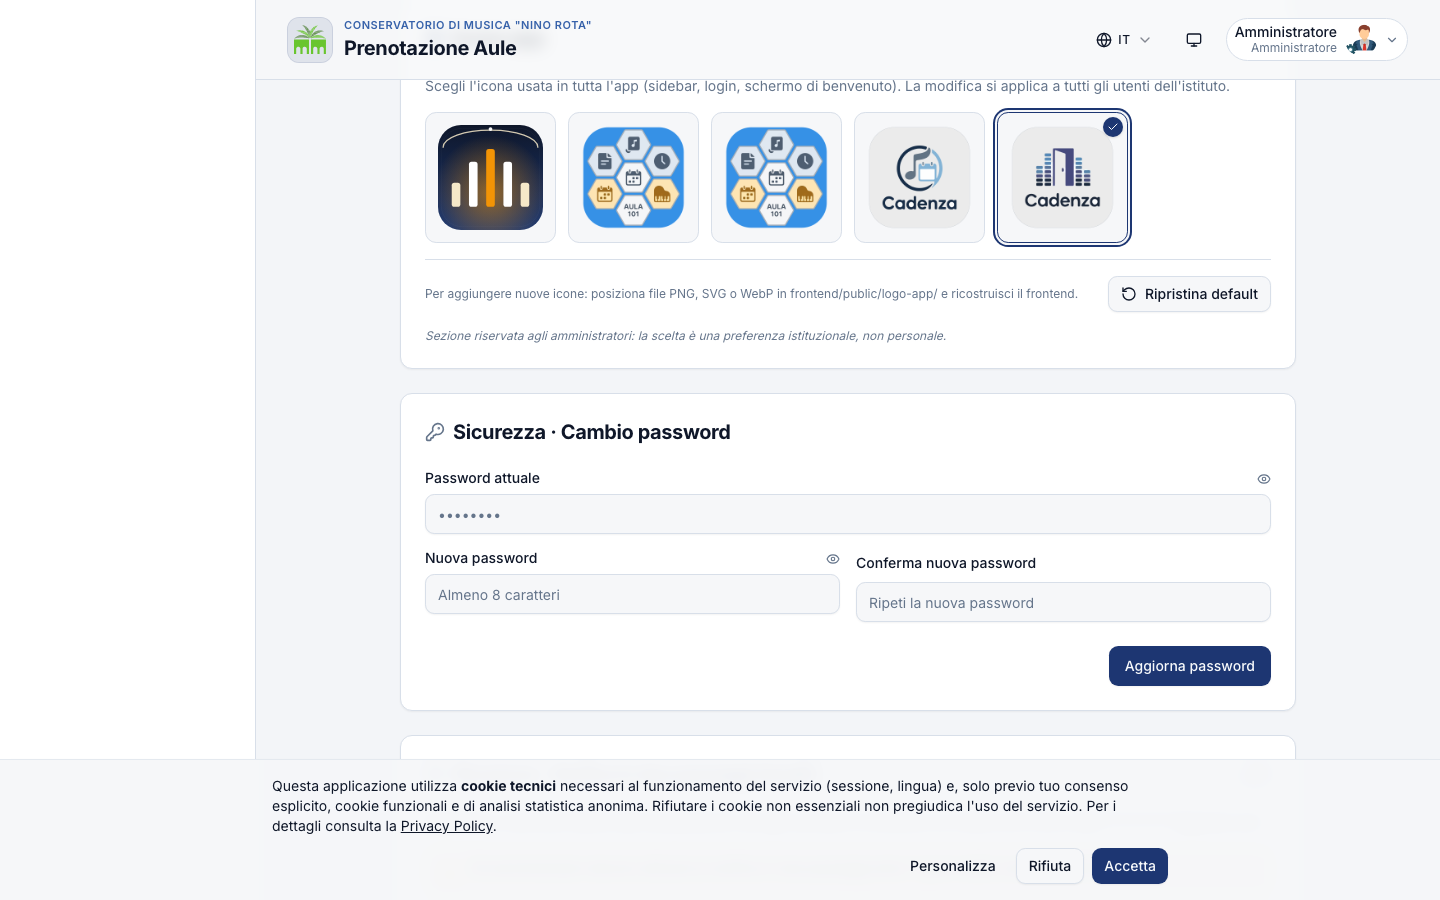
\includegraphics[width=0.95\linewidth]{screenshots/profile-app-icon.png}\caption*{Profilo — card "Aggiungi a Home" (PWA)}\end{figure}

\subsection{13.1 Installazione su Android}


\begin{enumerate}
  \item Apri Cadenza in Chrome.
  \item In alto a destra (tre puntini) $\rightarrow$ "Aggiungi a schermata Home" oppure usa il banner che compare automaticamente.
  \item L'icona Cadenza appare sulla home come un'app vera. Aprila: parte a tutto schermo, senza la barra del browser.
\end{enumerate}

\subsection{13.2 Installazione su iPhone (Safari)}


\begin{enumerate}
  \item Apri Cadenza in Safari.
  \item Tocca il pulsante "Condividi" (rettangolo con freccia in su).
  \item Scorri e tocca "Aggiungi a Home".
  \item Conferma. L'icona appare in home.
\end{enumerate}

\subsection{13.3 Offline-soft}


Quando il telefono perde rete, Cadenza non ti lascia "appeso":

\begin{itemize}
  \item Vedi un \textbf{banner giallo} in alto: "Connessione persa --- modalità offline".
  \item Le \textbf{pagine già visitate} restano leggibili (dashboard, le tue prenotazioni, profilo).
  \item Le \textbf{azioni che richiedono rete} (nuove prenotazioni, check-in, ecc.) sono temporaneamente disabilitate.
  \item Appena torna la rete il banner sparisce e tutto torna normale.
\end{itemize}

\begin{quote}
La modalità offline è soft: i dati sono cached, non scritti. Tutte le modifiche vere passano per il server.
\end{quote}

\medskip\hrule\medskip

\section{14. Bot Telegram (opzionale)}


\begin{quote}
\textbf{Cos'è}: un bot di Telegram con cui puoi prenotare, vedere le tue prenotazioni e ricevere promemoria \textbf{direttamente dalla chat}. Utile se hai sempre Telegram aperto e vuoi evitare il browser.
\end{quote}

Disponibile solo se la Direzione ha attivato l'integrazione.

\subsection{14.1 Setup (una volta sola)}


\begin{enumerate}
  \item In \texttt{/profile}, scorri fino alla card \textbf{"Bot Telegram"}.
  \item Cerca il bot del tuo Conservatorio su Telegram (la Direzione ti dice il nome, es. \texttt{@CadenzaConservatorioBot}).
  \item Avvia la chat e scrivi \texttt{/start}.
  \item Il bot ti chiede un \textbf{codice di binding} (OTP a 6 caratteri).
  \item Torna su \texttt{/profile} $\rightarrow$ "Genera codice" $\rightarrow$ copia il codice $\rightarrow$ incollalo nel bot.
  \item Bot e profilo Cadenza ora sono "legati".
\end{enumerate}

\subsection{14.2 Comandi disponibili}


\begin{table}[H]
\centering
\small
\begin{tabularx}{\linewidth}{|X|X|}
\hline
\rowcolor{tableheader} Comando & Cosa fa \\
\hline
\texttt{/aule} & Elenco aule prenotabili dal tuo ruolo \\
\hline
\texttt{/agenda} & Le tue prenotazioni dei prossimi 7 giorni \\
\hline
\texttt{/agenda 2026-11-12} & Snapshot di un giorno specifico (formato YYYY-MM-DD) \\
\hline
\texttt{/book} & Wizard a 5 step: sede $\rightarrow$ aula $\rightarrow$ quando $\rightarrow$ tipo $\rightarrow$ conferma \\
\hline
\texttt{/list} & Le tue prenotazioni future \\
\hline
\texttt{/cancel \textless{}id\textgreater{}} & Cancella la prenotazione con quell'ID \\
\hline
\texttt{/check \textless{}id\textgreater{}} & Effettua il check-in da remoto (solo se "vicino" all'aula in orario) \\
\hline
\texttt{/help} & Riepilogo comandi \\
\hline
\end{tabularx}
\end{table}


\subsection{14.3 Rate-limit}


Il bot ha un limite di \textbf{30 messaggi/minuto} e \textbf{200 messaggi/giorno} per utente. Sufficiente per uso normale, ti protegge da incidenti.

\medskip\hrule\medskip

\section{15. Lingue dell'interfaccia}


Cadenza è disponibile in \textbf{5 lingue}:

\begin{itemize}
  \item \textbf{IT} Italiano (default)
  \item \textbf{EN} English
  \item \textbf{ES} Español
  \item \textbf{DE} Deutsch
  \item \textbf{FR} Français
\end{itemize}

Cambia lingua dal menu in alto a destra (vicino al tuo nome). La preferenza viene memorizzata sul browser: la prossima volta ritrovi la lingua scelta.

\medskip\hrule\medskip

\section{16. Domande ricorrenti}


\textbf{Posso prenotare per un altro docente / per uno studente?} No, ogni prenotazione è legata al tuo account. Se devi farlo per ragioni operative (sostituzione, masterclass), parlane con il coordinatore: ha un comando admin apposito.

\textbf{Quante prenotazioni attive posso avere insieme?} Per i docenti il default è \textbf{20} prenotazioni future contemporanee. La Direzione può cambiare il limite. Lo vedi in \texttt{/my-bookings} con "5 / 20 attive".

\textbf{Ho dimenticato di fare check-in e l'aula è stata cancellata. Posso recuperare?} Sì: vai in \texttt{/booking}, ricrea la prenotazione per lo stesso slot. Se l'aula nel frattempo è stata presa da qualcun altro, scegli un'altra.

\textbf{Cosa succede se modifico una lezione dopo che è già stata "fatta"?} Non puoi: la modifica è bloccata per le prenotazioni passate o "checked-in". Lo storico è immutabile a fini di rendicontazione contabile.

\textbf{Il coordinatore mi ha "rifiutato" la proposta Monte Ore. Devo rifare tutto?} No, la proposta torna in \textbf{bozza} preservando tutte le tue fasce e celle. Apporti le modifiche richieste e re-invii. Vedi il motivo del rifiuto nel banner rosso.

\textbf{Ho 12 variazioni da fare in un anno ma il limite è 3. Cosa faccio?} Le \textbf{disattivazioni} (toggle off) NON consumano variazioni, sono sempre gratis. Solo le aggiunte/cambi orario/cambi aula/nuovi giorni consumano. Se ti servono davvero 12 modifiche strutturali, parlane con la Direzione: può sbloccare manualmente il contatore o intervenire in altro modo.

\textbf{Posso vedere le prenotazioni dei miei colleghi?} Sì, sulla Dashboard e sul calendario aule vedi tutti gli slot occupati (senza il nome del docente, per privacy --- solo "Occupato"). Il nome compare invece nella tua tab \texttt{/my-bookings} per le tue.

\textbf{Cadenza funziona se la rete del Conservatorio è giù?} Cadenza vive su un server cloud (Hetzner o equivalente), non sulla rete interna. Quindi sì, anche se la rete del Conservatorio è giù, da casa o dal cellulare 4G Cadenza funziona. L'unica eccezione è il \textbf{check-in QR}, che la Direzione può aver ristretto agli IP della rete interna.

\textbf{Chi vede i miei dati personali?} Solo tu, gli admin e --- limitatamente --- il coordinatore della didattica. Nessun dato è venduto/condiviso con terzi. Cadenza è ospitata in un datacenter europeo GDPR-compliant. Per il dettaglio leggi la pagina \textbf{Privacy} in fondo al sito.

\medskip\hrule\medskip

\textless{}div align="center"\textgreater{}

\textbf{Cadenza · La musica merita il software migliore}

\textit{© 2026 Danilo Russo · Manuale Docente v1.0 · 13 maggio 2026}

\textless{}/div\textgreater{}

\end{document}
